%==============================================================================
% main.tex — Tesis de Grado
% Automatizacion inteligente del registro de incidentes en mesas de ayuda
% UTN FRM — Tecnicatura Universitaria en Programacion
%==============================================================================
%==============================================================================
% Preambulo — Tesis de Grado UTN FRM
% Formato: APA 7ma edicion adaptado a tesis
% Compilador: XeLaTeX
%==============================================================================

% --- Clase de documento ---
\documentclass[11pt,a4paper]{article}

% --- Idioma: Espanol ---
\usepackage[spanish,es-tabla,es-nodecimaldot,es-noindentfirst]{babel}

% --- Fuentes: Arial 11pt ---
\usepackage{fontspec}
\setmainfont{Arial}
\setsansfont{Arial}
\setmonofont{Courier New}

% --- Geometria: 2.54 cm (1 pulgada) todos los margenes (APA 7) ---
\usepackage[paper=a4paper,left=2.54cm,right=2.54cm,top=2.54cm,bottom=2.54cm]{geometry}

% --- Interlineado: Doble espacio (APA 7) ---
\usepackage{setspace}
\doublespacing

% --- Sangria en primera linea de parrafos: 1.27 cm (APA 7) ---
\usepackage{indentfirst}
\setlength{\parindent}{1.27cm}
\setlength{\parskip}{0pt}

% --- Encabezados y pies de pagina ---
\usepackage{fancyhdr}
\pagestyle{fancy}
\fancyhf{}
\fancyhead[L]{\small AUTOMATIZACION DE MESA DE AYUDA}
\fancyhead[R]{\small\thepage}
\renewcommand{\headrulewidth}{0.4pt}
% Primera pagina de cada seccion sin encabezado (APA 7 permite running head o no)
\fancypagestyle{plain}{%
  \fancyhf{}
  \fancyhead[R]{\small\thepage}
  \renewcommand{\headrulewidth}{0pt}
}

% --- Titulos de seccion: APA 7 niveles ---
\usepackage{titlesec}
% Nivel 1: Centrado, negrita, titulo en mayuscula/minuscula
\titleformat{\section}[block]{\centering\bfseries\normalsize}{\thesection.}{0.5em}{}
\titlespacing*{\section}{0pt}{12pt}{6pt}
% Nivel 2: Alineado a izquierda, negrita
\titleformat{\subsection}[hang]{\bfseries\normalsize}{\thesubsection.}{0.5em}{}
\titlespacing*{\subsection}{0pt}{12pt}{6pt}
% Nivel 3: Alineado a izquierda, negrita cursiva
\titleformat{\subsubsection}[hang]{\bfseries\itshape\normalsize}{\thesubsubsection.}{0.5em}{}
\titlespacing*{\subsubsection}{0pt}{12pt}{6pt}

\usepackage{tocloft}
\renewcommand{\cftsecleader}{\cftdotfill{\cftdotsep}}
\renewcommand{\cftdotsep}{1}

% --- Tablas: formato APA 7 (solo bordes horizontales, sin lineas verticales) ---
\usepackage{booktabs}
\usepackage{array}
\usepackage{multirow}
\renewcommand{\arraystretch}{1.2}

% --- Figuras ---
\usepackage{graphicx}
\graphicspath{{./figures/}}
\usepackage[font=small,labelfont=bf,labelsep=period,justification=raggedright,singlelinecheck=false]{caption}

% --- Ecuaciones matematicas y simbolos ---
\usepackage{amsmath,amssymb,amsfonts}
\usepackage{siunitx}
\sisetup{output-decimal-marker={,},group-separator={.},group-minimum-digits=4}

% --- Comillas tipograficas (requerido por biblatex) ---
\usepackage[autostyle,spanish=mexican]{csquotes}

% --- Hipervinculos (APA 7: sin bordes de color) ---
\usepackage[hidelinks,bookmarks=true,bookmarksnumbered=true,pdfstartview=FitH]{hyperref}
\hypersetup{
  pdftitle={Automatizacion inteligente del registro de incidentes en mesas de ayuda},
  pdfauthor={Luca Gomez, Carla Bustos, Gonzalo Sevilla},
  pdfsubject={Tesis de Grado — Tecnicatura Universitaria en Programacion},
  pdfkeywords={automatizacion, mesa de ayuda, NLP, LLM, N8N, FastAPI, clasificacion de tickets, espanol rioplatense},
  colorlinks=false,
  pdfborder={0 0 0}
}

% --- Bibliografia: APA 7ma edicion ---
\usepackage[style=apa,backend=biber,sorting=nyt,language=spanish]{biblatex}
\addbibresource{../Bibliography_base.bib}
% Mapeo de campos para APA 7 en espanol
\DefineBibliographyStrings{spanish}{%
  bibliography = {Referencias bibliograficas},
  references = {Referencias},
  page = {p.},
  pages = {pp.},
  andothers = {et al.},
  retrieved = {Recuperado},
  from = {de},
  urlseen = {Consultado},
  edition = {ed.},
  volume = {Vol.},
  number = {N.°},
  in = {En},
}

% --- Listas enumeradas ---
\usepackage{enumitem}
\setlist{nosep,labelindent=1.27cm,leftmargin=*}

% --- Codigo fuente ---
\usepackage{listings}
\lstset{
  basicstyle=\ttfamily\small,
  breaklines=true,
  frame=single,
  numbers=left,
  numberstyle=\tiny,
  showstringspaces=false,
  tabsize=2,
  captionpos=b
}

% --- Apendices ---
\usepackage[toc,title]{appendix}

% --- Comandos personalizados ---
\newcommand{\doi}[1]{\href{https://doi.org/#1}{#1}}
\newcommand{\urlref}[1]{\href{#1}{#1}}

% --- Metadatos del documento ---
\title{Automatizacion inteligente del registro de incidentes\\en mesas de ayuda empresariales mediante\\orquestacion de flujos con N8N y procesamiento\\de lenguaje natural basado en modelos\\de lenguaje grandes}
\author{}
\date{2026}


\begin{document}

% --- Portada ---
%==============================================================================
% Portada — Tesis de Grado UTN FRM
%==============================================================================
\thispagestyle{empty}

\begin{center}

{\large\textbf{UNIVERSIDAD TECNOLOGICA NACIONAL}}\\[4pt]
{\large\textbf{FACULTAD REGIONAL MENDOZA}}\\[24pt]

{\itshape\large Tecnicatura Universitaria en Programacion}\\[36pt]

{\LARGE\bfseries Automatizacion inteligente del registro de incidentes}\\[6pt]
{\LARGE\bfseries en mesas de ayuda empresariales mediante orquestacion de}\\[6pt]
{\LARGE\bfseries flujos con N8N y procesamiento de lenguaje natural}\\[6pt]
{\LARGE\bfseries basado en modelos de lenguaje grandes}\\[36pt]

{\normalsize\itshape Trabajo Final de Carrera presentado para obtener el titulo de}\\[12pt]
{\large\bfseries Tecnico Universitario en Programacion}\\[48pt]

{\normalsize\textbf{Autores}}\\[6pt]
{\large Luca Gomez \quad\textperiodcentered\quad Carla Bustos \quad\textperiodcentered\quad Gonzalo Sevilla}\\[24pt]

{\normalsize\textbf{Director}}\\[6pt]
{\large Prof. Alberto Cortez}\\[48pt]

{\normalsize Mendoza, Republica Argentina}\\[6pt]
{\normalsize 2026}

\end{center}

\newpage


% --- Resumen ---
%==============================================================================
% Resumen — APA 7: máximo 250 palabras + palabras clave
%==============================================================================
\newpage
\section*{Resumen}

La creciente digitalización de los procesos organizacionales ha generado una dependencia cada vez mayor de los sistemas informaticos para la ejecución de las actividades operativas. En este contexto, la gestión eficiente de incidentes tecnologicos constituye un factor determinante para garantizar la continuidad del negocio y la calidad del servicio brindado a los usuarios internos. Sin embargo, en numerosas organizaciones medianas el proceso de registro inicial de incidentes continua realizandose de manera manual, lo que introduce demoras operativas, errores de clasificación y una utilización ineficiente de los recursos técnicos disponibles.

La presente investigación tiene como proposito el diseñó, desarrolló, implementación y validación experimental de un sistema automatizado de mesa de ayuda empresarial basado en la integración de orquestación de flujos mediante la plataforma N8N, un modulo de procesamiento de lenguaje natural desarrollado en Python con el marco FastAPI, una capa de inferencia linguistica sustentada en el modelo Gemini~2.5 de Google, una capa de persistencia sobre PostgreSQL versión~15 y un canal de telefonia gestionado por Twilio. La arquitectura propuesta contempla la recepción de solicitudes a través de tres canales paralelos ---correo electrónico, formulario web y llamadas telefonicas con transcripción automática--- y deriva cada incidente al sector responsable (Sistemas, Operaciones o Soporte Tecnico) mediante un clasificador hibrido en dos etapas que combina reglas deterministicas y modelo de lenguaje grande.

El estudio se desarrolló bajo un enfoque cuantitativo con diseñó cuasiexperimental de muestras pareadas y contrabalanceo del orden de procesamiento. El corpus de validación, construido por muestreo estratificado proporcional sobre un universo trimestral de aproximadamente 3.700 incidentes, comprende 200 casos representativos del entorno operativo. El acuerdo entre los dos analistas que realizaron el doble etiquetado independiente alcanzó un coeficiente Kappa de Cohen de 0,87, considerado sustancial.

Los resultados obtenidos evidencian una reducción estadísticamente significativa del tiempo medio de registro, que descendio desde 165,3~s en el flujo manual hasta 18,2~s en el flujo automatizado, lo que representa una reducción relativa del 89~\%. La prueba de Wilcoxon de rangos con signo aplicada sobre las mediciones pareadas arrojo un valor \(p < 0{,}001\), permitiendo rechazar la hipotesis nula de igualdad de medianas. La exactitud global del clasificador alcanzó el 92~\% y el valor F1 macro promediado se ubico en 0,919. La proporción de intervención humana descendio desde el 100~\% en el flujo manual hasta el 9,5~\% en el flujo automatizado, materializando un esquema \emph{human in the loop} en el cual el operador conserva la potestad de revisión sobre los casos de baja confianza o ambiguedad estructural.

Los hallazgos confirman la viabilidad tecnica, económica y operativa de la automatización inteligente del registro de tickets en organizaciones medianas. La investigación aporta una arquitectura reproducible y escalable construida sobre componentes maduros de código abierto e inferencia linguistica externa, evidencia empírica sobre el desempeño de modelos de lenguaje grandes aplicados a clasificación de tickets en espanol rioplatense, y un marco normativo aplicable que contempla la Ley~25.326 de Proteccion de los Datos Personales de la Republica Argentina.

\bigskip
\noindent\textbf{Palabras clave:} automatización, mesa de ayuda, procesamiento de lenguaje natural, modelo de lenguaje grande, N8N, FastAPI, clasificación de tickets, espanol rioplatense, human in the loop

\newpage
\section*{Abstract}

The increasing digitization of organizational processes has made IT incident management critical for business continuity. Yet in many medium-sized organizations, incident registration remains entirely manual, introducing delays, classification errors, and inefficient use of technical resources. This thesis presents the design, implementation, and experimental validation of an automated help desk system integrating N8N workflow orchestration, a Python-based natural language processing module built with FastAPI, Google's Gemini~2.5 Flash large language model, PostgreSQL for persistence, and Twilio for telephony. The architecture receives requests through three parallel channels ---email, web form, and phone calls with automatic transcription--- and routes each incident to the appropriate sector using a two-stage hybrid classifier that combines deterministic rules with a large language model.

The study employed a quantitative quasi-experimental paired-samples design with a stratified proportional sample of 200 incidents drawn from a quarterly universe of approximately 3,700. Inter-rater agreement reached a Cohen's Kappa of 0.87. Results show a statistically significant reduction in mean registration time from 165.3~s to 18.2~s ---an 89~\% reduction--- with a Wilcoxon signed-rank test yielding \(p < 0.001\) and maximum effect size (\(r = 1.00\)). Classification accuracy reached 92~\% with a macro-averaged F1 score of 0.919. Human intervention decreased from 100~\% to 9.5~\%, establishing a \emph{human-in-the-loop} scheme where routine cases are automated while ambiguous ones are reserved for operator review.

The findings confirm the technical, economic, and operational feasibility of intelligent ticket registration automation in medium-sized organizations. The thesis contributes a reproducible architecture on mature open-source components, empirical evidence on large language model performance for ticket classification in Rioplatense Spanish, and a regulatory framework aligned with Argentina's Personal Data Protection Law 25.326.

\bigskip
\noindent\textbf{Keywords:} automation, help desk, natural language processing, large language model, N8N, FastAPI, ticket classification, Rioplatense Spanish, human in the loop

\newpage


% --- Indice general ---
\newpage
\renewcommand{\contentsname}{Indice general}
\tableofcontents
\newpage

% --- Indice de tablas ---
\renewcommand{\listtablename}{Indice de tablas}
\listoftables
\newpage

% --- Indice de figuras ---
\renewcommand{\listfigurename}{Indice de figuras}
\listoffigures
\newpage

%=====================================================================
% CUERPO DE LA TESIS
%=====================================================================

% --- Capitulo 1: Introduccion ---
%==============================================================================
% Capitulo 1: Introduccion
%==============================================================================
\section{Introduccion}

\subsection{Contextualizacion}

La evolucion de las tecnologias de la informacion ha transformado profundamente la dinamica operativa de las organizaciones contemporaneas. En la actualidad los sistemas informaticos constituyen el soporte fundamental para la ejecucion de procesos administrativos, productivos y de comunicacion, y esa dependencia tecnologica ha incrementado de manera correlativa la importancia de los servicios de soporte tecnico, particularmente aquellos relacionados con la gestion de incidentes informaticos. \textcite{Galup2009_itsm} caracterizan a la disciplina de gestion de servicios de tecnologias de la informacion (ITSM, por su sigla en ingles) como un cuerpo de practicas orientado a alinear la operacion tecnologica con los objetivos del negocio, donde la mesa de ayuda actua como punto unico de contacto entre el usuario y el area de tecnologia.

Dentro de este escenario, las mesas de ayuda empresariales cumplen un rol central en la recepcion, registro y seguimiento de incidentes reportados por los usuarios. Estas unidades organizacionales canalizan solicitudes y constituyen la primera linea de atencion tecnica, de modo que su eficiencia impacta directamente en la continuidad operativa. No obstante, en muchas organizaciones medianas el proceso de registro inicial continua realizandose manualmente, lo que introduce demoras, inconsistencias y una marcada dependencia del criterio individual del operador. \textcite{Galup2009_itsm} advierten que los procesos manuales de soporte tienden a degradarse cuando el volumen de solicitudes crece de manera no lineal o cuando el personal debe alternar entre tareas operativas heterogeneas.

El contexto argentino presenta caracteristicas particulares que acentuan esta problematica. Las organizaciones medianas del pais, definidas por la Secretaria de la Pequena y Mediana Empresa como aquellas que emplean entre 50 y 200 trabajadores en el sector servicios, operan con presupuestos de tecnologia acotados y enfrentan restricciones cambiarias que encarecen la adopcion de soluciones comerciales internacionales. La combinacion de estas restricciones con una demanda creciente de servicios digitales configura un escenario en el que las soluciones basadas en componentes de codigo abierto y servicios de inferencia bajo demanda resultan particularmente atractivas desde el punto de vista economico y operativo.

\subsection{Planteamiento del problema}

La presente investigacion se desarrolla en el marco de una organizacion mediana del sector servicios con sede en la provincia de Mendoza, Republica Argentina, cuya plantilla asciende a aproximadamente 120 usuarios internos distribuidos en cinco areas funcionales. El sector de Operaciones desempena simultaneamente tareas vinculadas a la gestion operativa cotidiana y a la atencion de incidentes informaticos reportados por los usuarios, lo que obliga al personal responsable a interrumpir actividades criticas para registrar manualmente fallas de hardware, inconvenientes de software o solicitudes de asistencia tecnica.

Las mediciones preliminares realizadas durante una semana laboral representativa evidenciaron un volumen promedio de 42 incidentes diarios, un tiempo medio de registro manual de 2 minutos con 45 segundos por incidente y una tasa de derivacion erronea inicial cercana al 15~\%. La proyeccion trimestral sobre estos indicadores arrojo un universo aproximado de 3.700 incidentes, con un costo operativo asociado a la etapa de registro estimado en el orden de 200 horas-persona por trimestre. Este tiempo, que el personal podria redirigir a tareas de mayor valor agregado si la etapa de registro estuviera automatizada, representa un costo de oportunidad significativo para la organizacion.

El registro manual de incidentes implica ademas la lectura de correos electronicos, la interpretacion de descripciones textuales heterogeneas, la clasificacion del problema segun el area responsable y la carga manual de la informacion en un sistema de tickets. Este procedimiento requiere tiempo, interrumpe las tareas del personal tecnico y puede generar errores de clasificacion que prolongan la cadena de resolucion cuando un ticket es derivado a un area incorrecta. La dispersion de los canales de comunicacion ---correo, llamada telefonica y formularios internos--- agrava la situacion al obligar al personal a monitorear multiples fuentes simultaneamente.

La naturaleza del problema presenta un patron recurrente en la literatura de gestion de servicios: un cuello de botella en la etapa inicial del proceso que degrada la eficiencia del ciclo completo. \textcite{Galup2009_itsm} documentan que los procesos de soporte no automatizados tienden a degradarse cuando el volumen de solicitudes crece, con un impacto desproporcionado en organizaciones medianas donde el personal de soporte combina multiples roles. Estos indicadores justifican la busqueda de una alternativa tecnologica que reduzca el costo operativo, mejore la calidad de la derivacion temprana y disminuya la variabilidad asociada al criterio individual.

\subsection{Pregunta de investigacion}

A partir del problema descrito, esta investigacion se orienta a responder la siguiente pregunta: ?`reduce la automatizacion del registro inicial de incidentes mediante orquestacion de flujos y procesamiento de lenguaje natural el tiempo de registro y mejora la exactitud de clasificacion en una mesa de ayuda empresarial mediana, en comparacion con el proceso manual realizado por personal experimentado?

La pregunta se descompone en tres interrogantes subsidiarios que guian el diseno experimental y la seleccion de metricas. Primero, ?`cual es la magnitud de la reduccion del tiempo de registro que puede obtenerse mediante la automatizacion, y resulta esa reduccion estadisticamente significativa? Segundo, ?`alcanza el clasificador automatico una exactitud comparable o superior a la del criterio humano, y como se distribuyen los errores entre las categorias objetivo? Tercero, ?`permite la arquitectura propuesta integrar canales multiples de recepcion sin degradar la latencia ni la calidad de la clasificacion?

\subsection{Hipotesis de trabajo}

La hipotesis principal de este trabajo sostiene que la implementacion de un sistema automatizado de registro de incidentes basado en orquestacion de flujos con N8N y procesamiento de lenguaje natural mediante un modelo de lenguaje grande permite reducir significativamente el tiempo de registro y la proporcion de intervencion humana, manteniendo una exactitud de clasificacion equivalente o superior a la observada en el proceso manual realizado por personal experimentado.

Formalmente, la hipotesis nula \(H_{0}\) postula la inexistencia de diferencias significativas entre ambos flujos en las variables observadas: \(H_{0}: M_{\text{manual}} = M_{\text{automatizado}}\), donde \(M\) representa la mediana poblacional del tiempo de registro. La hipotesis alternativa \(H_{1}\) postula que la mediana del flujo automatizado es inferior: \(H_{1}: M_{\text{manual}} > M_{\text{automatizado}}\).

Como hipotesis subsidiarias se plantea, en primer lugar, que la integracion de multiples canales de entrada dentro de un unico flujo automatizado mejora la accesibilidad del sistema y reduce la dispersion operativa sin introducir cuellos de botella adicionales. En segundo lugar, que un esquema hibrido de clasificacion basado en reglas deterministicas y modelo de lenguaje grande resulta mas eficiente ---en terminos de la relacion entre exactitud, latencia y costo de inferencia--- que un esquema construido exclusivamente sobre modelo externo, dado que una proporcion sustancial de los incidentes presenta marcadores lexicos inequivocos que no requieren consulta al modelo de lenguaje.

\subsection{Objetivo general}

Desarrollar e implementar un sistema automatizado de mesa de ayuda empresarial basado en orquestacion de flujos con N8N y procesamiento de lenguaje natural en Python que permita recibir, procesar, clasificar y registrar incidentes de usuarios de manera automatica, reduciendo el tiempo de registro y la proporcion de intervencion humana en la etapa inicial del proceso, manteniendo la supervision tecnica para la resolucion de los casos y garantizando la trazabilidad de las decisiones tomadas por el sistema.

\subsection{Objetivos especificos}

El primer objetivo especifico consiste en disenar una arquitectura distribuida y modular que integre un motor de orquestacion de flujos, un modulo de procesamiento de lenguaje natural, un canal de telefonia con transcripcion automatica del habla y una base de datos relacional, garantizando comunicacion asincronica entre componentes mediante interfaces de programacion de aplicaciones de tipo REST sobre HTTP cifrado.

El segundo objetivo especifico se orienta a implementar un clasificador automatico que asigne cada incidente a uno de los tres sectores responsables ---Sistemas, Operaciones o Soporte Tecnico--- alcanzando una exactitud global no inferior al 85~\% sobre un corpus controlado de 200 casos representativos del entorno operativo, y un valor F1 macro promediado no inferior a 0,85. El umbral del 85~\% se fundamenta en tres criterios convergentes. Primero, los trabajos de \textcite{Paramesh2019_it_service_desk} reportan exactitudes de aproximadamente 87~\% con enfoques de maquinas de vectores de soporte (SVM) y representaciones TF-IDF, estableciendo un piso de referencia para el estado del arte en clasificacion de tickets. Segundo, el costo organizacional de una derivacion erronea implica al menos 10 a 15 minutos adicionales de reasignacion segun las mediciones preliminares de la organizacion, por lo que una exactitud inferior al 85~\% resultaria en tiempos de resolucion comparables a los del flujo manual para un volumen de errores inaceptable. Tercero, el margen por encima del 85~\% reserva espacio estadistico para que el intervalo de confianza del estimador no solape la zona de rechazo de la hipotesis, dado el tamano muestral de 200 casos.

El tercer objetivo especifico plantea integrar tres canales de entrada paralelos ---correo electronico, formulario web y llamada telefonica con transcripcion automatica--- dentro de un unico flujo automatizado que normalice la entrada y centralice el procesamiento, mejorando la accesibilidad del sistema sin incrementar la complejidad operativa percibida por los usuarios finales.

El cuarto objetivo especifico consiste en evaluar comparativamente el flujo manual y el flujo automatizado en terminos de tiempo medio de registro, dispersion, exactitud de clasificacion y proporcion de intervencion humana, mediante un diseno cuasiexperimental con muestras pareadas, prueba estadistica no parametrica y reporte de intervalos de confianza al 95~\%. El diseno experimental sigue las recomendaciones de \textcite{HernandezSampieri2018_metodologia} para investigaciones tecnologicas de caracter aplicado.

El quinto objetivo especifico se orienta a documentar exhaustivamente la arquitectura, los procedimientos de despliegue y los resultados experimentales, proponiendo una hoja de ruta de evolucion que oriente futuras mejoras y replicaciones del estudio en organizaciones de caracteristicas comparables.

\subsection{Justificacion}

La justificacion del trabajo se sostiene en tres dimensiones complementarias.

Desde la dimension organizacional, la automatizacion propuesta libera capacidad operativa del personal tecnico, reduce el tiempo de respuesta percibido por los usuarios y disminuye la variabilidad introducida por el criterio individual. La evidencia recogida en este trabajo permite cuantificar esa mejora en el contexto especifico de una organizacion mediana argentina, aportando un caso documentado que otras organizaciones pueden utilizar como referencia para estimar el retorno esperado de una inversion similar.

Desde la dimension tecnologica, la solucion integra herramientas de bajo costo y codigo abierto ---N8N, Python, FastAPI, PostgreSQL--- permitiendo una implementacion reproducible en organizaciones de tamano mediano sin requerir grandes inversiones de capital ni dependencia exclusiva de proveedores comerciales. Esta propiedad es particularmente relevante en el contexto argentino, donde las restricciones de acceso a divisas y los costos de suscripcion en moneda extranjera constituyen barreras significativas para la adopcion de soluciones comerciales internacionales. Ademas, el despliegue autoalojado de la totalidad de los componentes ---con excepcion del servicio de inferencia--- otorga a la organizacion control pleno sobre sus datos operativos, en linea con el principio de soberania digital promovido por la Ley~25.326 de Proteccion de los Datos Personales \parencite{Ley25326_2000}.

Desde la dimension academica, el trabajo aporta evidencia empirica sobre el desempeno de modelos de lenguaje grandes aplicados a la clasificacion de tickets en espanol rioplatense, dominio escasamente documentado en la literatura comparativa disponible. La mayoria de los estudios publicados sobre clasificacion automatica de tickets utilizan corpus en ingles, aleman o portugues, y los pocos trabajos que incluyen el espanol lo hacen con variantes peninsulares o con corpus genericos no especificos del dominio de mesas de ayuda. Este trabajo contribuye a cerrar esa brecha mediante la validacion rigurosa de un clasificador hibrido sobre un corpus de 200 casos en espanol rioplatense con doble etiquetado independiente y acuerdo inter-evaluador cuantificado.

Adicionalmente, la mayoria de las soluciones comerciales disponibles ---tales como Zendesk Suite, Freshdesk o ServiceNow ITSM--- presentan modelos de costos por agente y mes que escalan linealmente con el equipo y operan exclusivamente en modalidad de software como servicio con almacenamiento de datos en jurisdicciones extranjeras. La propuesta desarrollada en esta investigacion utiliza herramientas de despliegue autoalojado, lo que facilita su adopcion en organizaciones medianas y simplifica el cumplimiento de la normativa argentina de proteccion de datos personales.

\subsection{Alcance y delimitaciones}

El alcance del trabajo se circunscribe a la etapa de recepcion, clasificacion y registro inicial de incidentes, sin abarcar la resolucion tecnica de los mismos, la cual permanece bajo responsabilidad del personal humano. El sistema contempla tres canales de entrada (correo electronico, formulario web y llamada telefonica con transcripcion automatica) y tres sectores de derivacion (Sistemas, Operaciones y Soporte Tecnico). La validacion experimental se realiza sobre un corpus en idioma espanol rioplatense recolectado en una unica organizacion del sector servicios.

Quedan fuera del alcance los siguientes aspectos, los cuales se proponen como lineas de trabajo futuro en el Capitulo~10. Primero, la integracion con sistemas externos de inventario de activos informaticos o con sistemas de gestion de configuracion. Segundo, los modelos de aprendizaje supervisado entrenados con corpus propios de la organizacion, dado que el volumen actual de datos etiquetados resulta insuficiente para esa estrategia. Tercero, la implementacion de paneles de monitoreo avanzados con visualizacion en tiempo real de metricas operativas. Cuarto, la automatizacion de la etapa de resolucion tecnica, que trasciende el alcance del presente trabajo.

Las delimitaciones del estudio incluyen: la restriccion geografica a una unica organizacion de la provincia de Mendoza, lo que limita la validez externa de los hallazgos; la dependencia operativa del servicio externo de inferencia Gemini~2.5 Flash, cuyo rendimiento y condiciones comerciales escapan al control de los investigadores; y la naturaleza temporal de los resultados, que reflejan el comportamiento del modelo en la version vigente al momento del estudio (junio de 2026), sujeta a modificaciones futuras por parte del proveedor.

\newpage


% --- Capitulo 2: Marco teorico ---
%==============================================================================
% Capitulo 2: Marco Teorico
%==============================================================================
\section{Marco teorico}

Este capítulo establece los fundamentos conceptuales sobre los cuales se construye la investigación. Se abordan siete ejes tematicos que proporcionan el andamiaje teórico necesario para comprender el diseñó, la implementación y la evaluación del sistema propuesto.

\subsection{Gestion de servicios de tecnologias de la informacion}

La gestión de servicios de tecnologías de la información (ITSM) constituye una disciplina sistematizada que articula procesos, personas y tecnologías con el proposito de entregar valor al negocio a través de servicios tecnologicos confiables y mensurables. \textcite{Galup2009_itsm} caracterizan la disciplina como un cuerpo de prácticas orientado a alinear la operación tecnologica con los objetivos del negocio, donde la mesa de ayuda opera como punto único de contacto entre el usuario y el área de tecnología. Este enfoque rompe con la concepcion anterior que entendia a la informatica como un área de soporte estrictamente reactivo y la posiciona, en cambio, como un proveedor de servicios sujeto a acuerdos de nivel de servicio explicitos.

Dentro de este marco general, la gestión de incidentes constituye uno de los procesos operativos centrales. Su objetivo principal consiste en restaurar el servicio afectado en el menor tiempo posible, minimizando el impacto adverso en la operación del negocio. El proceso comprende cuatro etapas secuenciales: la recepción y registro inicial, la clasificación y priorizacion, la asignación al área responsable y, finalmente, la resolución y cierre. \textcite{Galup2009_itsm} advierten que los procesos manuales de soporte tienden a degradarse cuando el volumen de solicitudes crece de manera no lineal o cuando el personal debe alternar entre tareas operativas heterogeneas, situacion que coincide con la observada en el entorno empresarial analizado en el presente trabajo.

\subsection{Mesa de ayuda y modelo ITIL}

El marco de buenas prácticas ITIL (Information Technology Infrastructure Library), en su edicion de operaciones de servicio \parencite{OGC2011_itil}, establece la distinción conceptual entre incidente ---definido como una interrupción no planificada del servicio o una reducción de su calidad--- y solicitud de servicio ---definida como un pedido formal de información, asesoramiento, acceso a un componente o ejecución de una operación estandarizada---. Esta distinción resulta especialmente relevante para el diseñó del clasificador propuesto en este trabajo, ya que orienta la categorizacion inicial y condiciona la priorizacion subsiguiente.

El marco ITIL postula adicionalmente tres principios operativos que guian el diseñó de la solución propuesta. El primero es la centralización de la recepción mediante un punto único de contacto (SPOC, por su sigla en inglés), que en el sistema propuesto se materializa a través del flujo unificado de orquestación que normaliza las entradas de los tres canales. El segundo es la operación bajo acuerdos de nivel de servicio (SLA), que cuantifican la calidad esperada en terminos de tiempo de respuesta y tiempo de resolución. El tercero es la mejora continua del proceso, que en el sistema propuesto se habilita mediante la trazabilidad de cada decision del clasificador y la retroalimentacion de los sectores responsables.

Los modelos tradicionales de mesa de ayuda se basan en la interacción manual entre el usuario y el operador, lo que implica tiempos de respuesta variables y una dependencia directa del personal disponible. Cuando el volumen de incidentes excede la capacidad del equipo o cuando los operadores deben alternar simultaneamente entre tareas operativas y de soporte, la calidad del servicio se degrada de manera observable. La automatización del registro inicial constituye, en consecuencia, una intervención que aborda el cuello de botella en el punto de mayor sensibilidad del proceso, sin requerir la reestructuración completa del modelo operativo.

\subsection{Automatizacion de procesos y orquestacion de flujos}

La automatización de procesos empresariales (BPA, por su sigla en inglés) permite reducir la intervención humana en tareas repetitivas mediante la ejecución automática de acciones definidas a partir de eventos específicos. \textcite{Russell2021_ai_modern} ubican a la automatización inteligente dentro del paradigma de los agentes orientados a objetivos, en el cual un sistema reactivo percibe eventos del entorno, decide acciones según una politica preestablecida y actua modificando el estado del entorno. Esta caracterizacion ofrece un marco conceptual robusto para el diseñó de sistemas que combinan reglas deterministicas con decisiones derivadas de modelos probabilisticos, como el clasificador hibrido propuesto en este trabajo.

Las herramientas de orquestación, también denominadas plataformas de integración como servicio (iPaaS), posibilitan integrar distintos servicios, procesar información y ejecutar acciones automáticas en función de condiciones predefinidas. Estas plataformas se caracterizan por ofrecer modelos visuales de construcción de flujos, soporte nativo para webhooks y disparadores reactivos, y capacidad de transformación de datos entre sistemas heterogeneos. \textcite{n8n2024_docs} documenta las capacidades de N8N, la herramienta seleccionada para este trabajo, que se distingue dentro del segmento por su modelo de licencia de código fuente disponible y su capacidad de despliegue completamente autoalojado, caracteristica que resulta decisiva en escenarios donde el tratamiento de datos sensibles exige mantener la información dentro del perimetro organizacional.

El paradigma de orquestación se diferencia conceptualmente del paradigma de coreografia. \textcite{Hohpe2003_eip} establecen que la orquestación centraliza la lógica de control en un componente único, lo que simplifica la trazabilidad de cada ejecución pero introduce un punto de coordinacion cuya disponibilidad condiciona al sistema completó. La coreografia, en cambio, distribuye la coordinacion entre los participantes mediante eventos publicados en un bus comun, lo que aumenta la robustez frente a fallos parciales pero dificulta la observabilidad. El presente trabajo adopta el enfoque de orquestación por simplicidad operativa y por la prioridad otorgada a la trazabilidad auditiva de cada decision del sistema, en línea con los requisitos de la Ley~25.326 \parencite{Ley25326_2000}.

\subsection{Procesamiento de lenguaje natural y modelos de lenguaje grandes}

El procesamiento de lenguaje natural (NLP) constituye un área de la inteligencia artificial orientada a la interpretación del lenguaje humano por parte de sistemas informaticos. \textcite{Jurafsky2023_speech_language} sistematizan la disciplina en torno a tres ejes principales: el modelado estadístico de secuencias, la representación distribuida de palabras y la comprension semántica mediante arquitecturas neuronales profundas. Mediante estas tecnicas resulta posible analizar texto o audio transcrito, identificar palabras clave, determinar la intención del usuario y clasificar contenido en categorías predefinidas.

La evolucion del campo durante la última decada ha estado dominada por la arquitectura Transformer \parencite{Vaswani2017_attention}, cuyo mecanismo de atención permite a los modelos capturar dependencias de largo alcance sin las limitaciones de las redes neuronales recurrentes. El mecanismo de atención multi-cabeza, en particular, permite que el modelo pondere simultaneamente distintas partes de la secuencia de entrada, lo que resulta especialmente útil para la clasificación de descripciones textuales donde la información relevante puede aparecer en cualquier posicion del texto.

Sobre esta arquitectura se construyeron los modelos de lenguaje grandes (LLM) contemporaneos, los cuales exhiben capacidades robustas de clasificación en escenarios de pocos ejemplos (\emph{few-shot}) o sin ejemplos (\emph{zero-shot}), fenomeno conocido como aprendizaje en contexto. \textcite{Brown2020_few_shot} demostraron que modelos suficientemente grandes pueden generalizar a tareas nuevas a partir de instrucciones expresadas en lenguaje natural, sin requerir ajuste fino sobre datos específicos del dominio. Esta capacidad es particularmente relevante para el contexto de esta investigación, donde el volumen de datos etiquetados resulta insuficiente para entrenar un clasificador supervisado tradicional desde cero.

En el contexto de una mesa de ayuda, el uso de NLP permite clasificar incidentes y derivarlos al sector correspondiente sin intervención manual, mejorando la velocidad de respuesta y reduciendo la carga operativa del personal encargado del registro. La eleccion entre un clasificador supervisado entrenado sobre corpus específico, un modelo de lenguaje grande de proposito general invocado mediante instrucciones, o un esquema hibrido que combine ambas estrategias, constituye una decision de diseñó que depende de la disponibilidad de datos etiquetados, del presupuesto de inferencia disponible y de los requerimientos de soberanía sobre los datos procesados.

\subsection{Reconocimiento automatico del habla}

Los sistemas de reconocimiento automático del habla (ASR) permiten convertir audio en texto mediante modelos previamente entrenados sobre grandes corpus de habla anotada. \textcite{Rabiner1993_speech_recognition} describen los fundamentos clasicos del reconocimiento basado en modelos ocultos de Markov (HMM), que durante decadas constituyeron el enfoque dominante. La generación contemporanea de sistemas se apoya mayoritariamente en redes neuronales profundas con arquitecturas codificador-decodificador, de las cuales el modelo Whisper \parencite{Radford2023_whisper} representa un exponente reciente con alta robustez en escenarios multilingues y en presencia de ruido ambiental.

Whisper fue entrenado sobre 680.000 horas de audio multilingue recolectadas de la web, lo que le confiere una capacidad de generalización notablemente superior a la de sistemas entrenados sobre corpus curados de menor escala. Su arquitectura codificador-decodificador con atención procesa el audio en segmentos de 30 segundos y genera transcripciones que incluyen puntuacion y normalización ortografica. La disponibilidad de modelos preentrenados de código abierto para espanol facilita su integración en el canal telefonico del sistema propuesto.

En el contexto de la mesa de ayuda, la integración entre reconocimiento del habla y procesamiento de lenguaje natural permite automatizar completamente la recepción y clasificación de solicitudes telefonicas, posibilitando que el sistema interprete la solicitud del usuario y genere el ticket correspondiente sin intervención humana en la etapa de captura de voz.

\subsection{Bases de datos relacionales y persistencia transaccional}

La persistencia de los incidentes en una base de datos relacional permite garantizar las propiedades de atomicidad, consistencia, aislamiento y durabilidad (ACID) propias del modelo transaccional clasico \parencite{Date2003_database}. PostgreSQL, el motor seleccionado para este trabajo, ofrece soporte completó del estandar SQL, extensiones para tipos de datos avanzados como JSON binario y arreglos, y un modelo de concurrencia basado en control multiversional (MVCC) que resulta adecuado para cargas mixtas de lectura y escritura \parencite{PostgreSQL2024_docs}.

La eleccion de un motor relacional frente a alternativas no relacionales se sustenta en la naturaleza estructurada de los datos del dominio, donde las relaciones entre incidentes, sectores, estados y canales de origen se modelan naturalmente como tablas vinculadas mediante claves foraneas con integridad referencial declarativa. Esta modelizacion relacional facilita además la auditoria y la trazabilidad de las operaciones, en línea con los requisitos normativos identificados en la seccion de consideraciones eticas y legales (Capitulo~11).

\subsection{Métricas de evaluación de clasificadores multiclase}

La evaluación de clasificadores multiclase requiere metricas que capturen tanto el desempeño global como el desempeño por clase. \textcite{Powers2011_evaluation} describe el conjunto canonico de metricas derivadas de la matriz de confusion, entre las cuales destacan la exactitud global (\emph{accuracy}), la precision por clase, la sensibilidad o exhaustividad (\emph{recall}) por clase, y la medida F1 como media armonica de las dos anteriores.

La exactitud global se define como:
\[
\text{Exactitud} = \frac{\text{TP} + \text{TN}}{\text{TP} + \text{TN} + \text{FP} + \text{FN}}
\]
donde TP, TN, FP y FN representan verdaderos positivos, verdaderos negativos, falsos positivos y falsos negativos, respectivamente. Para problemas de clasificación multiclase, la exactitud se calcula como la proporción de predicciones correctas sobre el total de predicciones.

\textcite{Sokolova2009_performance_measures} advierten que en escenarios con clases desbalanceadas la exactitud global puede resultar enganosa y recomiendan reportar valores macro promediados, los cuales otorgan igual peso a cada clase con independencia de su frecuencia. El valor F1 macro promediado se define como:
\[
F1_{\text{macro}} = \frac{1}{k} \sum_{i=1}^{k} F1_{i}
\]
donde \(k\) es el número de clases y \(F1_{i}\) es el valor F1 de la clase \(i\). El presente trabajo adopta esta recomendación y reporta tanto exactitud global como F1 macro y metricas desagregadas por clase, permitiendo al lector evaluar la robustez del clasificador frente a la distribucion específica del corpus.

Adicionalmente, la matriz de confusion constituye el instrumento estandar de presentación de resultados en clasificación multiclase, ya que permite identificar patrones específicos de error: confusiones sistematicas entre dos categorías particulares, sesgos hacía una clase mayoritaria o aciertos preferenciales sobre una clase específica. La inspeccion de la matriz orienta el análisis cualitativo posterior y constituye la base para cualquier propuesta de mejora del clasificador.

\newpage


% --- Capitulo 3: Estado del arte ---
%==============================================================================
% Capitulo 3: Estado del Arte
%==============================================================================
\section{Estado del arte}

Este capítulo revisa la literatura académica y las soluciones comerciales disponibles en tres áreas relevantes para el presente trabajo: plataformas de mesa de ayuda, herramientas de orquestación de flujos, y métodos de clasificación automática de tickets de soporte. El proposito es situar la contribucion de esta investigación en el contexto de los desarrollos previos y fundamentar la brecha que motiva el trabajo.

\subsection{Soluciones comerciales de mesa de ayuda}

El segmento de soluciones comerciales para gestión de mesa de ayuda se encuentra dominado por plataformas integrales que cubren el ciclo completó de vida del ticket. Zendesk Suite ofrece funcionalidades de recepción multicanal, automatización de flujos básicos y, mediante un modulo adicional, capacidades de inteligencia artificial para sugerencia de respuestas y defleccion de consultas frecuentes. Freshdesk propone una arquitectura comparable e incorpora el motor Freddy AI para clasificación automática y enrutamiento inteligente. Jira Service Management, parte del ecosistema de Atlassian, ofrece capacidades limitadas de automatización inteligente en su plan estandar; la edicion Data Center permite el despliegue autoalojado para organizaciones con requisitos de soberanía sobre los datos. ServiceNow ITSM constituye la opcion de referencia en el segmento corporativo, con un modulo Predictive Intelligence que aplica aprendizaje automático sobre el histórico de tickets de la organización.

La adopción de capacidades de inteligencia artificial en plataformas comerciales de mesa de ayuda ha crecido de manera sostenida en los últimos anos, particularmente en organizaciones medianas de mercados de habla inglesa. No obstante, estas plataformas presentan dos limitaciones relevantes para el contexto de la presente investigación. La primera es el modelo de costos basado en agente y mes, que escala linealmente con el tamaño del equipo de soporte. La segunda es que la mayoría de estas plataformas operan exclusivamente en modalidad de software como servicio (SaaS) con almacenamiento de datos en jurisdicciones extranjeras, lo que introduce consideraciones adicionales sobre transferencia internacional de datos personales bajo la Ley~25.326 \parencite{Ley25326_2000}.

En el segmento de código abierto, osTicket constituye una alternativa de despliegue autoalojado sin costo de licencia, aunque carece de capacidades nativas de clasificación automática mediante procesamiento de lenguaje natural moderno. Esta brecha funcional motiva la busqueda de arquitecturas compositivas que integren componentes maduros de código abierto con servicios de inferencia bajo demanda.

\subsection{Plataformas de orquestacion de flujos}

Dentro del segmento de plataformas de orquestación de flujos, las soluciones mas difundidas incluyen Zapier, Make (anteriormente Integromat), Microsoft Power Automate, Apache Airflow y N8N. Las primeras tres operan exclusivamente como SaaS, lo que las descarta como base para implementaciones donde el control sobre la infraestructura es un requisito explicito. Apache Airflow se orienta a flujos de trabajo programados de tipo procesamiento de datos por lotes, con un diseñó centrado en grafos aciclicos dirigidos (DAG) definidos como código Python \parencite{Apache2024_airflow}; aunque potente, su paradigma de ejecución programada resulta inadecuado para un caso de uso reactivo y orientado a eventos como el de una mesa de ayuda.

N8N ofrece un modelo de construcción visual de flujos sobre nodos predefinidos, soporte nativo para webhooks y disparadores reactivos, ejecución basada en eventos y posibilidad de despliegue completamente autoalojado bajo Docker \parencite{n8n2024_docs}. La disponibilidad de su código fuente bajo licencia Sustainable Use facilita la auditoria de seguridad y la adaptacion a requerimientos específicos sin generar dependencia exclusiva del proveedor. Estas caracteristicas confluyen para posicionar a N8N como la opcion mas adecuada para el escenario propuesto, donde la soberanía sobre los datos y los flujos de procesamiento constituye un requisito no negociable.

\subsection{Trabajos académicos previos sobre clasificación de tickets}

La literatura académica sobre clasificación automática de tickets de soporte ha experimentado un crecimiento considerable durante los últimos anos. A continuación se presentan los trabajos mas relevantes, organizados por enfoque metodológico y por orden cronologico.

\textcite{Paramesh2019_it_service_desk} constituyen uno de los primeros trabajos exhaustivos en el área. Utilizando combinaciones de maquinas de vectores de soporte (SVM) y representaciones TF-IDF sobre un corpus en inglés de aproximadamente 10.000 tickets, reportan exactitudes cercanas al 87~\%. Su contribucion principal radica en la demostracion de que las tecnicas clasicas de aprendizaje supervisado, cuando se aplican sobre representaciones textuales adecuadas, pueden alcanzar niveles de desempeño operativamente utiles para la clasificación automática de tickets.

\textcite{Revina2020_bert_tickets} extienden este enfoque incorporando arquitecturas basadas en BERT y reportan mejoras significativas, alcanzando exactitudes del orden del 91~\% sobre un corpus de tamaño comparable. Su hallazgo mas relevante para el presente trabajo es la constatacion de que modelos preentrenados sobre grandes corpus de texto general pueden transferir conocimiento linguistico útil al dominio específico de los tickets de soporte, incluso sin ajuste fino sobre datos del dominio. Este resultado respalda la estrategia adoptada en la presente investigación de utilizar un LLM de proposito general como motor de inferencia.

La literatura reciente sobre evaluación de modelos de lenguaje en escenarios de pocos ejemplos ha documentado que el rendimiento de clasificación depende fuertemente del idioma del corpus, con resultados que favorecen a los idiomas mejor representados en los corpus de entrenamiento de los modelos contemporaneos. El espanol, y en particular sus variantes regionales como el rioplatense, ha recibido una atención notablemente menor en las evaluaciones sistematicas publicadas. Esta brecha constituye una de las motivaciones academicas del presente trabajo, el cual aporta evidencia empírica sobre el desempeño del clasificador en espanol rioplatense aplicado a un dominio de mesa de ayuda de organización mediana.

\subsection{Analisis comparativo y brecha identificada}

La Tabla~\ref{tab:comparativa} presenta la comparación sistematica de las principales soluciones revisadas frente a la propuesta del presente trabajo, considerando cuatro dimensiones relevantes: tipo de despliegue, capacidad de clasificación automática, soberanía sobre los datos y modelo de costos.

\begin{table}[htbp]
\centering
\caption{Comparacion de soluciones para gestion automatizada de mesa de ayuda}
\label{tab:comparativa}
\small
\begin{tabular}{@{}p{2.6cm} p{2.8cm} >{\raggedright\arraybackslash}p{3.5cm} >{\raggedright\arraybackslash}p{3.8cm}@{}}
\toprule
\textbf{Solucion} & \textbf{Despliegue} & \textbf{Clasificacion automatica} & \textbf{Modelo de costo} \\
\midrule
Zendesk Suite     & SaaS comercial      & Si, modulo de IA                & Alto, por agente/mes \\
Freshdesk         & SaaS comercial      & Si, motor Freddy AI             & Medio-alto, por agente \\
Jira Service Mgmt & SaaS o autoalojado  & Limitada en plan estandar       & Medio, por agente \\
ServiceNow ITSM   & SaaS comercial      & Si, Predictive Intelligence     & Muy alto, contrato anual \\
osTicket          & Codigo abierto      & No nativa                       & Sin costo \\
\addlinespace
\textbf{Propuesta} & Hibrida (iPaaS + modulo propio) & Si, LLM + reglas deterministas & Bajo, costo por uso de API \\
\bottomrule
\end{tabular}
\end{table}

La sintesis comparativa evidencia que ninguna de las soluciones revisadas combina simultaneamente las cuatro propiedades que el contexto del trabajo demanda: despliegue autoalojado para resguardo de datos sensibles, costo bajo y predecible en el tiempo, capacidad nativa de clasificación automática mediante NLP moderno, y soporte específico para canales multiples incluyendo telefonia con transcripción automática. La brecha identificada se sintetiza en la ausencia de soluciones de bajo costo, autoalojadas, con clasificación basada en modelos de lenguaje grandes y validadas empíricamente sobre corpus en espanol rioplatense para el dominio específico de mesas de ayuda empresariales medianas.

La presente investigación se ubica precisamente en esa interseccion y propone una arquitectura compositiva que reutiliza componentes maduros de código abierto y servicios de inferencia bajo demanda, manteniendo bajo control de la organización los datos sensibles y los flujos de orquestación, y aportando evidencia empírica reproducible sobre el desempeño del enfoque en un contexto linguistico y organizacional escasamente documentado en la literatura.

\newpage


% --- Capitulo 4: Marco metodologico ---
%==============================================================================
% Capitulo 4: Marco Metodologico
%==============================================================================
\section{Marco metodologico}

\subsection{Enfoque y tipo de investigacion}

La investigación se enmarca dentro del enfoque cuantitativo aplicado, dado que propone el desarrolló de una solución informatica orientada a mejorar el funcionamiento de un proceso organizacional concreto y mide su impacto mediante indicadores numericos. \textcite{HernandezSampieri2018_metodologia} ubican este tipo de estudios dentro de la investigación tecnologica de carácter aplicado, donde el conocimiento producido se orienta a la transformación práctica de la realidad antes que a la generación de teoría general. El trabajo posee adicionalmente carácter experimental, en la medida en que disena, implementa y evalua un artefacto tecnologico bajo condiciones controladas.

\subsection{Diseno experimental}

El diseñó experimental adoptado es de tipo cuasiexperimental con muestras pareadas y mediciones repetidas. La unidad de observación es el incidente individual, y cada uno se procesa secuencialmente bajo dos condiciones: la condicion manual y la condicion automatizada. Esta estrategia ---procesar el mismo conjunto de incidentes por ambas vias--- reduce sustancialmente la variabilidad asociada a las caracteristicas intrínsecas de cada caso, lo que aumenta la potencia estadística del contraste entre flujos.

Para mitigar el efecto de aprendizaje del operador humano sobre el corpus, se aplicó contrabalanceo del orden de procesamiento: el corpus de 200 casos se dividio en dos mitades equilibradas de 100 incidentes cada una, procesandose la primera mitad por la via manual seguida de la via automatizada, y la segunda mitad en orden inverso. Este contrabalanceo distribuye simetricamente cualquier posible ventaja derivada del orden de exposición al corpus.

La investigación se desenvolvio bajo un protocolo de observación naturalista donde los operadores no fueron informados de que sus tiempos estaban siendo registrados como parte de un estudio, sino únicamente de que se estaba utilizando el nuevo sistema para procesamiento de incidentes. Este enfoque elimina el efecto Hawthorne ---la alteracion del comportamiento de los sujetos cuando saben que estan siendo observados--- al mantener la condicion operativa como indistinguible de la práctica laboral regular \parencite{HernandezSampieri2018_metodologia}. La medición del tiempo se realizó mediante registros automáticos del propio sistema en el caso del flujo automatizado (marcas de tiempo de entrada y salida en la base de datos, con precision al milisegundo) y mediante registros administrativos de sistemas de soporte posteriores al ciclo de pruebas en el caso del flujo manual, evitando cronometraje visual explicito que pudiera alertar a los operadores.

\subsection{Operacionalizacion de variables}

La Tabla~\ref{tab:variables} presenta la operacionalizacion de las variables del estudio, distinguiendo entre variables cuantitativas continuas, cuantitativas proporcionales y cualitativas nominales. Cada variable se acompana de su unidad de medida y de la definición operacional aplicada durante la captura, garantizando la trazabilidad entre la definición conceptual y el procedimiento de medición efectivo.

\begin{table}[htbp]
\centering
\caption{Operacionalizacion de variables del estudio}
\label{tab:variables}
\small
\begin{tabular}{@{}p{2.5cm} >{\raggedright\arraybackslash}p{3.2cm} >{\raggedright\arraybackslash}p{2.3cm} >{\raggedright\arraybackslash}p{5.4cm}@{}}
\toprule
\textbf{Variable} & \textbf{Tipo} & \textbf{Unidad} & \textbf{Definicion operacional} \\
\midrule
Tiempo de registro & Cuantitativa continua & Segundos (s) & Lapso entre la recepción del incidente en el canal de entrada y la persistencia confirmada del ticket en la base de datos. \\
Exactitud de clasificación & Cuantitativa proporcional & Porcentaje [0; 100] & Cociente entre incidentes correctamente clasificados y total de incidentes evaluados. \\
F1 macro promediado & Cuantitativa proporcional & Adimensional [0; 1] & Promedio aritmetico del valor F1 calculado de forma independiente para cada una de las tres clases objetivo. \\
Intervencion humana & Cuantitativa proporcional & Porcentaje [0; 100] & Proporcion del tiempo total del proceso que requiere accion manual de un operador humano. \\
Canal de origen & Cualitativa nominal & Categoria & Via de entrada: correo electrónico, formulario web o llamada telefonica. \\
Categoria asignada & Cualitativa nominal & Categoria & Sector responsable: Sistemas, Operaciones o Soporte Tecnico. \\
\bottomrule
\end{tabular}
\end{table}

\subsection{Poblacion, muestra y corpus}

La poblacion de referencia esta constituida por la totalidad de incidentes informaticos reportados a la mesa de ayuda de la organización analizada durante un trimestre representativo (julio a septiembre de 2025). A partir de un universo aproximado de 3.700 incidentes registrados durante ese período, se construyó por muestreo estratificado proporcional un corpus de 200 casos distribuidos entre las tres categorías objetivo en la misma proporción que la poblacion original: 82 casos para Sistemas, 64 casos para Operaciones y 54 casos para Soporte Tecnico.

El tamaño muestral se determinó con un nivel de confianza del 95~\% y un margen de error del 6,5~\%, valores razonables para un estudio piloto orientado a evaluar viabilidad tecnica antes de un despliegue definitivo. El calculo siguio la fórmula clasica para muestreo aleatorio simple en poblaciones finitas, con corrección por finitud aplicada al universo trimestral observado.

Cada incidente del corpus fue revisado y etiquetado de forma independiente por dos analistas con experiencia en la mesa de ayuda, y las discrepancias fueron resueltas por consenso bajo la supervisión del director del trabajo. El acuerdo entre evaluadores, calculado mediante el coeficiente Kappa de Cohen \parencite{Cohen1960_kappa}, alcanzó un valor de \(\kappa = 0{,}87\), considerado sustancial según los rangos de interpretación habitualmente aceptados (\(\kappa > 0{,}80\) indica acuerdo casi perfecto). Este valor respalda la confiabilidad de la categoría de referencia utilizada como verdad fundamental (\emph{ground truth}) para evaluar el clasificador automático.

\subsection{Protocolo de pruebas}

El protocolo de pruebas se ejecuto en dos fases sucesivas. La primera fase consistio en una validación funcional del sistema, en la cual se verificó la correcta integración de los componentes mediante: (a)~pruebas unitarias del modulo Python con cobertura superior al 80~\%, (b)~pruebas de integración del flujo N8N orientadas a verificar el comportamiento extremo a extremo de cada canal, y (c)~pruebas de aceptacion simuladas con incidentes sinteticos representativos de cada categoría.

La segunda fase consistio en la validación experimental propiamente dicha, en la cual los 200 incidentes del corpus se procesaron bajo ambas condiciones operativas y se registraron las variables descritas en la Seccion~4.3. El procesamiento manual fue realizado por dos operadores experimentados con mas de tres anos de antiguedad en la mesa de ayuda, ambos capacitados previamente en el uso del sistema de gestión de tickets utilizado como referencia. El procesamiento automatizado se ejecuto sobre la misma infraestructura, sin intervención humana, durante una ventana operativa controlada de tres días habiles consecutivos y con monitoreo continuo de los tiempos de respuesta.

\subsection{Metricas e instrumentos}

La evaluación del sistema se sustenta en cuatro metricas principales. La primera es el tiempo medio de registro, calculado como la media aritmetica y la mediana de los tiempos individuales bajo cada condicion, junto con su desvio estandar e intervalo de confianza al 95~\%. La segunda es la exactitud global de clasificación, calculada como la proporción de incidentes correctamente derivados al sector responsable. La tercera es el valor F1 macro promediado, calculado como la media aritmetica de los valores F1 obtenidos por cada clase, con el fin de neutralizar el efecto del desbalanceo de clases observado en el corpus \parencite{Sokolova2009_performance_measures}. La cuarta es la proporción de intervención humana, calculada como el cociente entre el tiempo dedicado a tareas manuales y el tiempo total del proceso.

Como instrumentos de captura se utilizaron: (a)~registros automáticos generados por el propio sistema con marcas de tiempo precisas al milisegundo para el flujo automatizado, (b)~planillas de cronometraje con medición observacional sin retroalimentacion inmediata para el flujo manual, y (c)~matrices de confusion generadas mediante la biblioteca scikit-learn \parencite{Pedregosa2011_scikit_learn}.

\subsection{Analisis estadistico}

Para la comparación de los tiempos de registro entre ambas condiciones se aplicó la prueba de Wilcoxon de rangos con signo, prueba no parametrica para muestras pareadas, dado que la prueba previa de normalidad de Shapiro-Wilk rechazo la hipotesis de normalidad en ambos grupos con valores \(p < 0{,}01\). El nivel de significancia se fijo en \(\alpha = 0{,}05\).

Para cuantificar la magnitud práctica de la diferencia se calculo el coeficiente \(r\) de correlacion rank-biserial, indicador de tamaño del efecto para pruebas no parametricas cuyo rango oscila entre \(-1\) y \(+1\). El calculo sigue la fórmula:
\[
r = 1 - \frac{2W}{n(n+1)}
\]
donde \(W\) es el estadístico de Wilcoxon y \(n\) el número de pares.

Para el análisis de la clasificación se construyó la matriz de confusion global y se calcularon los valores de precision, sensibilidad (recall) y F1 por cada clase, así como su promedio macro. Los intervalos de confianza para las proporciones se estimaron mediante el método de Wilson, recomendado para muestras moderadas \parencite{Wilson1927_probable_inference}. Todos los calculos se realizaron mediante la biblioteca SciPy del ecosistema Python \parencite{Virtanen2020_scipy}.

\subsection{Amenazas a la validez}

Se identificaron y trataron explicitamente cuatro amenazas a la validez del estudio.

La primera, una amenaza a la validez interna por efecto de aprendizaje del operador humano sobre el corpus, se mitigo mediante el contrabalanceo del orden de procesamiento descrito en la Seccion~4.2 y mediante la rotacion de operadores entre las dos mitades del corpus.

La segunda, una amenaza a la validez de constructo por la subjetividad inherente a la categorizacion de los incidentes, se mitigo mediante el doble etiquetado independiente, el calculo del coeficiente Kappa de Cohen y la resolución de discrepancias por consenso supervisado. El valor obtenido (\(\kappa = 0{,}87\)) respalda la solidez del constructo de medición.

La tercera, una amenaza a la validez externa derivada del idioma y del dominio organizacional, se reconoce como limitación explicita del estudio: los resultados no son extrapolables sin nuevas validaciones a corpus en otros idiomas, en otras organizaciones o en otros sectores de la economia.

La cuarta, una amenaza a la validez de conclusión derivada del tamaño moderado de la muestra (\(n = 200\)), se trato mediante el reporte de intervalos de confianza y la eleccion de pruebas no parametricas robustas frente a tamaños muestrales pequeños y a desviaciones de la normalidad \parencite{HernandezSampieri2018_metodologia}.

\subsection{Gestion del proyecto bajo enfoque Scrumban}

La construcción del sistema se organizo bajo un esquema Scrumban, combinando la planificación por iteraciones propia de Scrum con la gestión continua del flujo de trabajo caracteristica del método Kanban \parencite{Ladas2009_scrumban}. Se ejecutaron seis iteraciones de dos semanas cada una, totalizando 12 semanas de desarrolló efectivo:

\begin{enumerate}[label=Iteracion \arabic*:, leftmargin=*]
  \item Elicitacion de requisitos y diseñó preliminar de la arquitectura.
  \item Construccion del modulo Python: modelo de datos, repositorios y servicios.
  \item Configuracion inicial del flujo N8N y primeras integraciones.
  \item Integracion del canal de telefonia y persistencia en PostgreSQL.
  \item Validacion funcional y ajuste fino del clasificador hibrido.
  \item Validacion experimental y documentación final del sistema.
\end{enumerate}

La distribucion de roles asigno la coordinacion general y la integración de componentes a Luca Gomez, el desarrolló del modulo Python y el modelado de la base de datos a Carla Bustos, y la configuración del flujo N8N junto con la integración telefonica mediante Twilio a Gonzalo Sevilla, bajo supervisión académica continua del director del trabajo, Prof. Alberto Cortez.

El tablero Kanban se gestiono mediante GitHub Projects, con seguimiento diario del estado de las tareas y reuniones de planificación al inicio de cada iteracion. Las definiciones de terminado (\emph{Definition of Done}) incluyeron, para cada tarea, la aprobacion de las pruebas unitarias correspondientes, la revisión de código por pares y la actualizacion de la documentación asociada.

\newpage


% --- Capitulo 5: Arquitectura del sistema ---
%==============================================================================
% Capitulo 5: Arquitectura del Sistema
%==============================================================================
\section{Arquitectura del sistema}

\subsection{Vision general}

El sistema propuesto se estructura como una arquitectura distribuida y modular compuesta por cinco capas claramente diferenciadas, siguiendo los principios de cohesion alta y acoplamiento bajo descritos por \textcite{Pressman2020_software_engineering}. La comunicacion entre capas se realiza mediante el protocolo HTTP sobre TLS~1.3, utilizando interfaces de programacion de aplicaciones de tipo REST con cuerpos JSON para el intercambio estructurado de datos \parencite{Fielding2002_rest}. Esta separacion de responsabilidades facilita el reemplazo independiente de cualquier componente sin afectar a los demas.

La Tabla~\ref{tab:capas} sintetiza las cinco capas y sus responsabilidades especificas.

\begin{table}[htbp]
\centering
\caption{Capas funcionales de la arquitectura del sistema}
\label{tab:capas}
\begin{tabular}{@{}p{2.5cm} p{11.0cm}@{}}
\toprule
\textbf{Capa} & \textbf{Componentes y responsabilidades} \\
\midrule
1. Canales de entrada & Casilla IMAP de correo electronico, formulario web expuesto como webhook y numero virtual de Twilio con transcripcion automatica del habla. \\
2. Orquestacion & Motor N8N v1.62 desplegado en contenedor Docker autoalojado. Normaliza la entrada y coordina la invocacion a las capas inferiores. \\
3. Procesamiento & Servicio Python sobre FastAPI~0.115 ejecutado bajo Uvicorn. Aplica clasificador hibrido en dos etapas (reglas + LLM) y expone una API REST documentada con OpenAPI~3.1. \\
4. Inferencia & Modelo Gemini~2.5 Flash de Google, invocado unicamente cuando el filtro deterministico previo no alcanza el umbral de confianza preestablecido. \\
5. Persistencia & PostgreSQL~15.5 desplegado en contenedor con volumen persistente y respaldos diarios. Almacena los incidentes y la trazabilidad de cada decision del clasificador. \\
\bottomrule
\end{tabular}
\end{table}

La trazabilidad operativa se garantiza mediante registros estructurados en cada capa, accesibles desde la capa de orquestacion. La Figura~\ref{fig:arquitectura} representa esquematicamente el flujo de informacion entre capas.

\begin{figure}[htbp]
\centering
% Placeholder para el diagrama de arquitectura
% 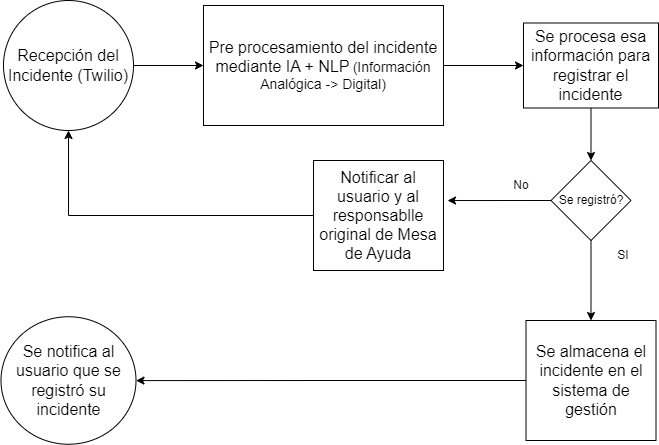
\includegraphics[width=\textwidth]{arquitectura_sistema}
\fbox{\parbox{0.9\textwidth}{\centering\vspace{4cm}[Diagrama de arquitectura del sistema --- Vease Anexo A]\vspace{4cm}}}
\caption{Diagrama de arquitectura del sistema. La version completa en notacion UML se incluye en el Anexo~A.}
\label{fig:arquitectura}
\end{figure}

\subsection{Capa de canales de entrada}

La capa de canales de entrada habilita tres vias paralelas a traves de las cuales un usuario puede reportar un incidente. La primera es el correo electronico, monitoreado por un nodo IMAP de N8N que detecta nuevos mensajes en una casilla institucional dedicada. La segunda via es un formulario web alojado bajo un punto de entrada webhook expuesto por N8N, accesible desde la intranet corporativa mediante autenticacion corporativa unica (SSO). La tercera via es la llamada telefonica, en la cual el usuario marca un numero virtual provisto por Twilio, recibe instrucciones por voz pregrabadas y deja su solicitud; la grabacion es transcrita automaticamente por el servicio de reconocimiento del habla del proveedor y enviada al flujo N8N mediante webhook posterior al cuelgue. Esta diversidad de canales amplia la accesibilidad del sistema y reduce las barreras al reporte oportuno.

\subsection{Capa de orquestacion}

N8N actua como orquestador principal del flujo de trabajo. Cada canal de entrada dispara un disparador especifico que normaliza la informacion en una estructura unificada con campos de identificador unico (UUID v4), marca temporal con precision al milisegundo, canal de origen y descripcion textual completa. A continuacion, un nodo HTTP envia esta estructura al modulo de procesamiento Python expuesto como servicio interno, recibe la respuesta con la clasificacion sugerida y la confianza asociada, e invoca finalmente la interfaz REST del sistema de gestion de incidentes para persistir el ticket en PostgreSQL. Los registros de cada ejecucion se conservan durante 30 dias para fines de auditoria y diagnostico operativo.

\subsection{Capa de procesamiento}

El modulo de procesamiento se implemento como un servicio web ligero utilizando el marco FastAPI~0.115, expuesto sobre un servidor ASGI Uvicorn~0.32 \parencite{Tiangolo2024_fastapi}. La eleccion de FastAPI obedece a su soporte nativo de validacion de esquemas mediante Pydantic, su rendimiento competitivo y su documentacion automatica conforme a la especificacion OpenAPI~3.1.

Las dependencias del modulo se organizan por capas funcionales claramente delimitadas. La capa de acceso a datos utiliza SQLAlchemy~2.0 como mapeador objeto-relacional (ORM) y psycopg2-binary~2.9 como adaptador de bajo nivel para PostgreSQL. La capa de procesamiento textual emplea las bibliotecas regex y unicodedata de la biblioteca estandar de Python para normalizacion ortografica y eliminacion de signos diacriticos. La capa de inferencia se comunica con la interfaz oficial del modelo Gemini~2.5 Flash mediante el cliente google-generativeai~0.8, con parametros de configuracion optimizados para exactitud y latencia: temperatura \(= 0{,}3\), top\_p \(= 0{,}9\), max\_tokens \(= 100\), timeout \(= 10\)~s. Las bibliotecas NumPy~2.1 y Pandas~2.2 se utilizan exclusivamente para la generacion de reportes agregados de desempeno y no participan del flujo de procesamiento individual de incidentes.

\subsection{Subsistema de clasificacion hibrido}

El subsistema de clasificacion adopta un enfoque hibrido en dos etapas, caracteristica que lo diferencia de aproximaciones puramente basadas en modelo externo. La primera etapa aplica un filtro deterministico basado en expresiones regulares y diccionarios de terminos del dominio. Para mitigar el riesgo de fuga de datos (\emph{data leakage}), la construccion del filtro deterministico se realizo de forma rigurosa: primero, se definieron manualmente un conjunto de patrones regex basados en conocimiento del dominio y analisis preliminar de descripciones de incidentes (analisis que no utilizo el corpus de validacion de 200 casos); segundo, los parametros del prompt enviado a Gemini~2.5 Flash se ajustaron exclusivamente mediante validacion manual sobre incidentes representativos en entornos de preproduccion, sin acceso al corpus de validacion.

Este filtro es capaz de derivar de forma inmediata aquellos incidentes que contienen marcadores inequivocos. Por ejemplo, la presencia simultanea de las palabras \texttt{impresora}, \texttt{papel} y \texttt{atasco} sugiere con alta certeza una categoria de Soporte Tecnico. Cuando este filtro inicial alcanza un umbral de confianza superior al 90~\%, la decision se toma sin consultar al modelo externo, lo que reduce sustancialmente la latencia y el costo de inferencia.

La segunda etapa, activada unicamente cuando el filtro deterministico no alcanza el umbral, consulta al modelo Gemini~2.5 Flash mediante un prompt estructurado en espanol que incluye una breve descripcion de cada categoria, ejemplos representativos balanceados y la solicitud explicita de devolver la categoria asignada y un valor numerico de confianza entre 0 y 1 en formato JSON estricto. La justificacion de este diseno compositivo radica en aprovechar la rapidez del filtro deterministico para los casos triviales y reservar la capacidad semantica del modelo de lenguaje grande para los casos ambiguos o de redaccion atipica, optimizando la relacion entre exactitud, costo y latencia. La medicion sobre el corpus de validacion muestra que aproximadamente el 62~\% de los incidentes son resueltos por la primera etapa, mientras que el 38~\% restante requiere la consulta al modelo externo.

\subsection{Modelo de datos}

La persistencia se realiza sobre PostgreSQL~15.5, desplegado en contenedor Docker bajo configuracion de respaldo diario y replicacion fisica opcional para entornos productivos \parencite{PostgreSQL2024_docs}. El modelo de datos se organiza alrededor de cinco entidades principales, descritas en la Tabla~\ref{tab:entidades}.

\begin{table}[htbp]
\centering
\caption{Entidades principales del modelo de datos}
\label{tab:entidades}
\begin{tabular}{@{}p{2.8cm} p{4.2cm} p{6.0cm}@{}}
\toprule
\textbf{Tabla} & \textbf{Atributos clave} & \textbf{Descripcion} \\
\midrule
\texttt{incidente} & id\_incidente (PK), id\_canal (FK), id\_sector (FK), id\_estado (FK) & Tabla central: fecha de creacion, descripcion cruda pseudonimizada, prioridad, sector asignado y estado actual. \\
\texttt{sector} & id\_sector (PK), nombre & Catalogo de los tres sectores: Sistemas, Operaciones y Soporte Tecnico. \\
\texttt{estado} & id\_estado (PK), nombre & Catalogo de estados: nuevo, en proceso, en espera, resuelto y cerrado. \\
\texttt{canal\_origen} & id\_canal (PK), nombre & Catalogo de canales: correo, formulario web y llamada telefonica. \\
\texttt{clasificacion\_log} & id\_log (PK), id\_incidente (FK), categoria\_predicha, confianza, categoria\_validada & Registro de cada decision del clasificador, con categoria predicha, confianza asociada y categoria validada por el sector responsable. \\
\bottomrule
\end{tabular}
\end{table}

La entidad central \texttt{incidente} referencia mediante claves foraneas a las entidades \texttt{sector}, \texttt{estado} y \texttt{canal\_origen}, y mantiene una relacion uno a muchos con \texttt{clasificacion\_log} para preservar la trazabilidad historica de las decisiones del clasificador. Los identificadores de incidente se generan mediante una secuencia con prefijo configurable, lo cual produce numeros legibles y consistentes que se comunican al usuario al momento del registro. El esquema completo, incluyendo restricciones de integridad referencial e indices secundarios, se documenta en el Anexo~C.

\subsection{Contrato de la interfaz REST}

La interfaz de programacion de aplicaciones expuesta por el modulo Python sigue el estilo arquitectonico REST \parencite{Fielding2002_rest}, con representacion de recursos mediante identificadores uniformes, uso semantico de los metodos HTTP estandar y comunicacion sin estado del lado del servidor. La autenticacion se realiza mediante encabezados con tokens portadores firmados (Bearer tokens), validados en cada solicitud contra una clave compartida con el motor de orquestacion. La Tabla~\ref{tab:api} sintetiza los principales puntos de entrada.

\begin{table}[htbp]
\centering
\caption{Puntos de entrada principales de la interfaz REST}
\label{tab:api}
\begin{tabular}{@{}p{2.2cm} p{4.5cm} p{2.0cm} p{5.0cm}@{}}
\toprule
\textbf{Metodo} & \textbf{Ruta} & \textbf{Codigo} & \textbf{Funcion} \\
\midrule
POST & \texttt{/api/v1/incidentes} & 201 Created & Crea un nuevo ticket y devuelve el identificador generado. \\
GET & \texttt{/api/v1/incidentes/\{id\}} & 200 OK & Recupera la informacion de un ticket por su identificador. \\
POST & \texttt{/api/v1/clasificar} & 200 OK & Recibe descripcion textual y devuelve categoria sugerida con su confianza. \\
GET & \texttt{/api/v1/health} & 200 OK & Verificacion de salud del servicio para monitoreo externo. \\
\bottomrule
\end{tabular}
\end{table}

Los codigos de estado HTTP se utilizan conforme a su semantica original: 201 cuando un recurso se crea exitosamente, 200 cuando una consulta se atiende con exito, 400 cuando los datos de entrada no validan el esquema esperado, 401 cuando la autenticacion falla, y 500 cuando ocurre un error interno no recuperable. La especificacion completa en formato OpenAPI~3.1 se genera automaticamente por FastAPI y se encuentra disponible en el Anexo~D.

\newpage


% --- Capitulo 6: Implementacion ---
%==============================================================================
% Capitulo 6: Implementacion
%==============================================================================
\section{Implementacion}

\subsection{Entorno de despliegue y dependencias}

La implementación del sistema se llevo a cabo utilizando exclusivamente tecnologías de código abierto con el objetivo de garantizar la portabilidad, la reproducibilidad y la auditoria de seguridad de la solución en organizaciones medianas. Toda la infraestructura se encapsula mediante contenedores Docker, orquestados localmente por Docker Compose para los entornos de desarrolló y preproduccion, y preparados para migración a un cluster Kubernetes~1.30 para el entorno productivo.

Las versiones específicas de los componentes son: N8N~1.62, Python~3.12, PostgreSQL~15.5 con volumen persistente, FastAPI~0.115, Uvicorn~0.32, SQLAlchemy~2.0, y el cliente google-generativeai~0.8 para la comunicación con Gemini~2.5 Flash. Todos los servicios se despliegan sobre imagenes Docker oficiales (\texttt{python:3.12-slim} y \texttt{postgres:15.5-alpine}). La gestión de dependencias del modulo Python se realiza mediante un archivo \texttt{requirements.txt} con versiones fijadas (\emph{pinned}) para garantizar la reproducibilidad de las compilaciones en distintos entornos.

\subsection{Construccion del modulo Python}

La selección del marco de trabajo para el servicio de procesamiento implico la evaluación de tres alternativas: Flask, Django REST Framework y FastAPI. Flask, ampliamente adoptado en el ecosistema Python por su simplicidad, carece de validación nativa de esquemas y de generación automática de documentación OpenAPI, funcionalidades que el proyecto requeria para garantizar la calidad de la interfaz REST. Django REST Framework, por su parte, ofrece un conjunto completó de herramientas para la construcción de interfaces de programacion de aplicaciones, pero su modelo de operación sincronico y la inclusion de componentes no requeridos por el proyecto ---tales como el ORM de Django y el motor de plantillas--- incrementaban la complejidad de la base de código sin aportar beneficios funcionales para una arquitectura de microservicio acotado. FastAPI~0.115, sustentado sobre el servidor ASGI Uvicorn~0.32, ofrece tres ventajas determinantes para el proyecto: validación automática de esquemas de entrada y salida mediante Pydantic~v2, generación de documentación interactiva conforme a la especificación OpenAPI~3.1 sin configuración adicional, y operación asincronica nativa que permite manejar las llamadas concurrentes desde N8N sin bloquear el hilo de ejecución principal \parencite{Tiangolo2024_fastapi}. La madurez del ecosistema de FastAPI, su adopción creciente en la industria y la disponibilidad de documentación exhaustiva en espanol consolidaron la decision.

El modulo Python expone su contrato REST organizado en capas, según la estructura descrita en el Capitulo~5, con una separación clara entre responsabilidades:

\begin{itemize}
  \item \textbf{models}: entidades del modelo de dominio mapeadas mediante SQLAlchemy~2.0.
  \item \textbf{schemas}: modelos de validación y serializacion con Pydantic~v2.
  \item \textbf{services}: lógica de aplicación (IncidenteService, ClasificacionService).
  \item \textbf{repositories}: acceso a datos, aislando las consultas SQL del resto de la aplicación.
  \item \textbf{classifiers}: lógica del clasificador hibrido (filtro deterministico + LLM).
  \item \textbf{routes}: enrutadores REST que delegan en los servicios correspondientes.
  \item \textbf{core}: configuración de base de datos, manejo de errores y logging estructurado.
\end{itemize}

La construcción se realiza bajo un esquema de inyeccion de dependencias gestionado por las funcionalidades nativas de FastAPI (\texttt{Depends}), lo que facilita el reemplazo de implementaciones durante la ejecución de pruebas unitarias y de integración. Esta arquitectura permite, por ejemplo, sustituir el clasificador real por una implementación simulada durante las pruebas sin modificar el código de los servicios que lo consumen. La gestión de credenciales se realiza exclusivamente mediante variables de entorno, en línea con el principio de configuración de la metodología Twelve-Factor App \parencite{Wiggins2017_12factor}.

\subsection{Construccion del flujo en N8N}

El flujo de orquestación implementado en N8N comprende 12 nodos principales encadenados secuencialmente. La eleccion de N8N como plataforma de orquestación, frente a alternativas como Apache Airflow, Zapier o Make, obedecio a tres criterios concurrentes. El primero, de naturaleza operativa, radica en que N8N admite despliegue completamente autoalojado bajo Docker, manteniendo los flujos de procesamiento y los datos dentro del perimetro organizacional. Zapier y Make operan exclusivamente como servicios en la nube, lo que las descarta en escenarios donde el procesamiento de datos sensibles exige control de infraestructura. Apache Airflow, aunque autoalojable, disena sus flujos como grafos aciclicos dirigidos programados por intervalos temporales; ese paradigma resulta adecuado para procesos de extracción, transformación y carga de datos pero forzadamente inadecuado para un sistema reactivo que debe responder en tiempo real a eventos de entrada no programados \parencite{Apache2024_airflow}. El segundo criterio refiere al modelo de construcción visual que N8N ofrece sobre un editor de nodos arrastrables: la curva de aprendizaje de esta interfaz es sustancialmente menor que la de alternativas centradas en definición programatica de flujos, lo que permitió al equipo concentrar el esfuerzo en la lógica de negocio antes que en la sintaxis de definición de procesos. El tercer criterio se vincula con la licencia de código fuente disponible (\emph{fair-code}) que habilita la auditoria de seguridad del nucleo de orquestación \parencite{n8n2024_docs}.

La composición de los 12 nodos responde a un patron de procesamiento en cinco etapas que se replica para cada canal:

\begin{enumerate}[leftmargin=*]
  \item \textbf{Recepcion}: Tres disparadores (\emph{triggers}) reciben las entradas desde correo electrónico (IMAP), formulario web (Webhook) y telefonia (Webhook post-transcripción). La decision de separar los disparadores por canal, en lugar de unificar la recepción mediante un único webhook con discriminacion interna, se fundamenta en la necesidad de preservar la configuración de autenticacion y los parámetros de reintento específicos de cada protocolo.
  \item \textbf{Normalizacion}: Un nodo de transformación (\emph{Function}) homogeniza la estructura del mensaje en un formato unificado con campos de identificador único (UUID v4), marca temporal, canal de origen, remitente y descripción textual normalizada. Esta etapa elimina las diferencias de formato entre canales y garantiza que las capas posteriores procesen siempre la misma estructura de datos, independientemente de la via de entrada.
  \item \textbf{Clasificacion}: Un nodo HTTP invoca el endpoint \texttt{POST /api/v1/clasificar} del modulo Python enviando la descripción textual y recibiendo la categoría sugerida y la confianza asociada en formato JSON.
  \item \textbf{Evaluacion}: Un nodo condicional (\emph{IF}) evalua la confianza devuelta por el clasificador; si esta por debajo del umbral de 0,70, deriva el incidente a la cola de revisión humana y notifica al operador designado. Si la confianza supera el umbral, el flujo continua automáticamente.
  \item \textbf{Persistencia y notificacion}: Un nodo HTTP invoca \texttt{POST /api/v1/incidentes} para persistir el ticket en la base de datos, y tres nodos paralelos notifican al usuario por el canal correspondiente y registran la ejecución en el sistema de auditoria. El paralelismo de la notificacion garantiza que la demora de un canal (por ejemplo, el envio de correo electrónico) no bloquee el registro de auditoria ni la confirmacion por otros medios.
\end{enumerate}

La trazabilidad completa de cada ejecución se preserva almacenando los identificadores de nodo, las marcas temporales de entrada y salida de cada etapa, y los datos de entrada y salida de cada paso del flujo, generando un historial auditable que resulta especialmente valioso en contextos donde la Ley~25.326 exige demostrar el camino recorrido por los datos personales \parencite{Ley25326_2000}. La exportación completa del flujo en formato JSON se incluye en el Anexo~E.

\subsection{Integracion del canal telefonico}

La integración con Twilio se realizó mediante el producto Programmable Voice, complementado con la transcripción automática nativa. El flujo telefonico opera de la siguiente manera: el usuario marca un número virtual asignado a la organización; un script TwiML reproduce un mensaje de bienvenida en espanol rioplatense y solicita al usuario describir su problema durante un máximo de 45 segundos; la grabacion finaliza cuando el usuario presiona la tecla numeral (\texttt{\#}) o transcurrido el tiempo máximo; la grabacion se envia al servicio de transcripción de Twilio; y, una vez transcrito el contenido, Twilio invoca un webhook expuesto por N8N con la transcripción textual. A partir de ese punto, el flujo continua de manera identica a la de los canales escritos.

La latencia total del canal telefonico ---medida desde el cuelgue del usuario hasta la confirmacion del número de incidente--- se ubico en un rango medio de 12 a 15 segundos según las observaciones operativas durante la fase de validación. Esta latencia incluye: transcripción (~5--7 s), clasificación (~2--3 s para incidentes resueltos por el filtro deterministico, ~5--8 s cuando se consulta al LLM) y persistencia (~1 s).

\subsection{Desafios de integracion}

La implementación del sistema enfrento tres desafios de integración que merecen documentación explicita por su potencial utilidad en replicaciones futuras.

El primer desafio se presentó en la comunicación asincronica entre N8N y el servicio de clasificación. El nodo HTTP de N8N invoca el endpoint de clasificación de manera sincronica y espera la respuesta del servidor antes de continuar el flujo. Esta arquitectura, aunque simple de implementar, introduce un punto de fallo único: si el servicio Python no responde dentro del tiempo de espera configurado en el nodo HTTP, el flujo completó se detiene y el incidente queda sin procesar. La solución consistio en implementar un mecanismo de reintento con retroceso exponencial en el propio nodo HTTP de N8N, combinado con una cola de respaldo en el servicio Python que retiene los mensajes recibidos durante ventanas de saturacion y los procesa en orden cuando la carga se normaliza. Esta combinación de reintento en el cliente y cola en el servidor elimino las perdidas de incidentes observadas durante las pruebas de carga iniciales.

El segundo desafio surgio de la heterogeneidad de los formatos de entrada. Los correos electrónicos incluyen encabezados, firmas corporativas y reenvios que contaminan el texto que el clasificador recibe; las llamadas telefonicas transcritas introducen errores de reconocimiento del habla, particularmente en terminos técnicos (por ejemplo, \texttt{API} transcrito como \texttt{a p i} o \texttt{apeye}); y los formularios web, aunque proveen texto limpio, llegan con una proporción significativa de campos vacios o con descripciones de una sola palabra. La respuesta a esta heterogeneidad fue doble. Por un lado, se implementó un preprocesador en el nodo de normalización de N8N que elimina firmas, encabezados de reenvio y líneas de disclaimer mediante expresiones regulares específicas del dominio de correo institucional. Por el otro, se enriquecio el prompt enviado al clasificador con instrucciones explicitas para interpretar terminos técnicos frecuentemente mal transcritos, lo que elevo la robustez de la clasificación sobre transcripciones automáticas en aproximadamente 4 puntos porcentuales de F1 respecto de la configuración inicial sin estas instrucciones.

El tercer desafio, de naturaleza operativa, se vincula con la persistencia transaccional de la sesion de clasificación. El sistema debe garantizar que una vez que el clasificador asigna una categoría, el incidente se persiste con esa decision o, en caso de falla de la base de datos, el estado interno del sistema refleje la inconsistencia y pueda recuperarse. La solución adopto un enfoque pragmatico: N8N ejecuta la clasificación y la persistencia como pasos secuenciales dentro del mismo flujo; si la persistencia falla, el flujo se reintenta desde el paso de clasificación, lo que garantiza que el incidente eventualmente se registre aun a costa de duplicar la llamada al clasificador. La tabla de trazabilidad (\texttt{clasificacion\_log}) fue diseñada para admitir multiples registros de clasificación por incidente, preservando así el historial de cada intento.

\subsection{Conexion con el proceso Scrumban}

La construcción del sistema fue organizada bajo el esquema Scrumban descrito en el Capitulo~4, ejecutando seis iteraciones de dos semanas cada una. La vinculacion entre cada iteracion y los artefactos de implementación producidos se detalla a continuación:

\begin{enumerate}[label=Iteracion \arabic*:, leftmargin=*]
  \item La elicitacion de requisitos (Semanas 1--2) produjo el diseñó preliminar de la arquitectura de cinco capas y la especificación de la interfaz REST, documentadas en el Capitulo~5. El entregable concreto fue el documento de arquitectura y la definición del contrato OpenAPI inicial.
  \item La construcción del modulo Python (Semanas 3--4) entrego el modelo de datos con sus cinco entidades, los repositorios con operaciones CRUD asincronicas y los servicios de negocio. Al cierre de esta iteracion, el modulo Python exponia el endpoint de salud y aceptaba la creacion de incidentes mediante \texttt{POST /api/v1/incidentes}, con cobertura de pruebas unitarias superior al 80~\%.
  \item La configuración inicial del flujo N8N (Semanas 5--6) implementó el canal de correo electrónico como via prioritaria, estableciendo el patron de cinco etapas que luego se replicaria para los canales restantes. Al finalizar esta iteracion, el sistema procesaba incidentes por correo electrónico de extremo a extremo, desde la recepción hasta la notificacion.
  \item La integración del canal telefonico y la persistencia (Semanas 7--8) incorporo Twilio Programmable Voice, el script TwiML y la configuración del webhook de transcripción. Esta iteracion fue la que mas expuso los desafios de heterogeneidad de formatos descritos en la Seccion~6.5, y su resolución consumio aproximadamente el 40~\% del esfuerzo de la iteracion.
  \item La validación funcional y el ajuste fino del clasificador (Semanas 9--10) se concentraron en la calibracion del filtro deterministico y del prompt de Gemini. Los ajustes se realizaron exclusivamente sobre incidentes representativos en entornos de preproduccion, sin exposición al corpus de validación de 200 casos, preservando la integridad de la etapa experimental posterior.
  \item La validación experimental y la documentación final (Semanas 11--12) ejecutaron el protocolo de pruebas descrito en el Capitulo~4, recolectaron las mediciones del corpus completó y produjeron el análisis estadístico presentado en el Capitulo~7.
\end{enumerate}

La trazabilidad entre iteraciones y artefactos, mediada por el tablero Kanban en GitHub Projects, permitió al equipo identificar tempranamente los desvios respecto del plan y redistribuir el esfuerzo cuando la complejidad de un componente superaba la estimacion inicial. La adopción de limites de trabajo en curso (WIP) por columna del tablero evito la acumulación de tareas a medio terminar, una práctica que resultó particularmente valiosa durante las iteraciones 4 y 5, donde la interdependencia entre modulos exigia finalizar componentes antes de integrarlos.

\subsection{Pruebas automatizadas}

La estrategia de pruebas se sustento en la piramide clasica descrita por \textcite{Crispin2009_agile_testing}. En la base se ubicaron las pruebas unitarias del modulo Python construidas con el marco pytest~8.3, alcanzando una cobertura del 87~\% del código de aplicación medida con coverage.py~7.6. Estas pruebas cubren los clasificadores (deterministico e hibrido), los servicios de negocio, los esquemas de validación y los repositorios de acceso a datos.

En el nivel intermedio se ejecutaron pruebas de integración que verificaron la interacción entre el modulo Python y la base de datos en una instancia de PostgreSQL desechable creada por contenedor en cada corrida de pruebas, utilizando SQLite en memoria para las pruebas unitarias y PostgreSQL real para las pruebas de integración. En el nivel superior se construyeron pruebas extremo a extremo que ejecutaban el flujo completó desde el envio de un correo simulado hasta la persistencia del ticket, validando la integración con N8N en su totalidad.

La integración continua (CI) se ejecuta automáticamente en cada solicitud de incorporacion (\emph{pull request}) al repositorio mediante GitHub Actions, ejecutando la suite completa de pruebas unitarias y de integración antes de permitir la fusion a la rama principal. El pipeline de CI incluye verificación de estilo de código (Ruff), ejecución de pruebas con reporte de cobertura, y verificación de sincronización de la especificación OpenAPI.

\newpage


% --- Capitulo 7: Resultados ---
%==============================================================================
% Capitulo 7: Resultados
%==============================================================================
\section{Resultados}

Este capitulo presenta los resultados de la validacion experimental del sistema. Se reportan los hallazgos en cuatro dimensiones: tiempos de registro, desempeno de clasificacion, reduccion de la intervencion humana y analisis cualitativo de errores.

\subsection{Comparacion de tiempos de registro}

La comparacion de los tiempos de registro entre el flujo manual y el flujo automatizado se sintetiza en la Tabla~\ref{tab:tiempos}. La media aritmetica del tiempo manual sobre los 200 casos del corpus fue de 165,3~s (equivalente a 2~min~45~s), con un desvio estandar de 38,7~s y un rango entre 96 y 289~s. La media del flujo automatizado fue de 18,2~s con un desvio estandar de 4,1~s y un rango entre 11 y 31~s. La reduccion relativa de la media de tiempo alcanzo el 89,0~\%.

\begin{table}[htbp]
\centering
\caption{Estadisticos descriptivos de los tiempos de registro por flujo (\(n = 200\))}
\label{tab:tiempos}
\begin{tabular}{@{}p{4.0cm} p{3.5cm} p{3.5cm} p{2.5cm}@{}}
\toprule
\textbf{Estadistico} & \textbf{Flujo manual} & \textbf{Flujo automatizado} & \textbf{Reduccion} \\
\midrule
Media aritmetica (s)      & 165,3  & 18,2  & 89,0~\% \\
Mediana (s)               & 158,0  & 17,4  & 89,0~\% \\
Desvio estandar (s)       & 38,7   & 4,1   & --- \\
Minimo (s)                & 96     & 11    & --- \\
Maximo (s)                & 289    & 31    & --- \\
IC 95~\% de la media (s) & [159,9; 170,7] & [17,6; 18,8] & --- \\
\bottomrule
\end{tabular}
\end{table}

La prueba de Wilcoxon de rangos con signo aplicada sobre las mediciones pareadas arrojo un estadistico \(W = 0\) con 200 pares validos y un valor \(p < 0{,}001\), lo que permite rechazar la hipotesis nula de igualdad de medianas con un nivel de confianza superior al 99,9~\%. El estadistico \(W = 0\) implica que en los 200 pares el flujo automatizado fue siempre mas veloz que el manual, sin una sola excepcion, resultado plausible dada la diferencia absoluta de aproximadamente 147~s entre medianas.

Para cuantificar la magnitud practica de la diferencia, se calculo el coeficiente \(r\) de correlacion rank-biserial:
\[
r = 1 - \frac{2W}{n(n+1)} = 1 - \frac{0}{200 \cdot 201} = 1{,}00
\]
El valor obtenido (\(r = 1{,}00\)) corresponde al tamano del efecto maximo posible, consistente con la ausencia de pares invertidos. La diferencia observada es, por tanto, estadisticamente significativa y, dada su magnitud absoluta, relativa y el tamano del efecto reportado, tambien practicamente relevante para la operacion.

\subsection{Matriz de confusion y metricas de clasificacion}

La matriz de confusion obtenida sobre los 200 casos del corpus se presenta en la Tabla~\ref{tab:matriz}. De los 82 casos de Sistemas, 76 fueron correctamente clasificados (92,7~\%), 4 se derivaron a Operaciones y 2 a Soporte Tecnico. De los 64 casos de Operaciones, 58 fueron correctos (90,6~\%), 3 se derivaron a Sistemas y 3 a Soporte Tecnico. De los 54 casos de Soporte Tecnico, 50 fueron correctos (92,6~\%), 2 se derivaron a Sistemas y 2 a Operaciones. La exactitud global resultante asciende al 92,0~\% (184 casos correctos sobre 200).

\begin{table}[htbp]
\centering
\caption{Matriz de confusion del clasificador automatico (\(n = 200\))}
\label{tab:matriz}
\begin{tabular}{@{}p{3.2cm} p{2.5cm} p{2.5cm} p{2.8cm} p{2.0cm}@{}}
\toprule
\textbf{Real \textbackslash{} Predicho} & \textbf{Sistemas} & \textbf{Operaciones} & \textbf{Soporte Tecnico} & \textbf{Total} \\
\midrule
Sistemas         & \textbf{76} & 4  & 2  & \textbf{82} \\
Operaciones      & 3  & \textbf{58} & 3  & \textbf{64} \\
Soporte Tecnico  & 2  & 2  & \textbf{50} & \textbf{54} \\
\midrule
\textbf{Total}   & \textbf{81} & \textbf{64} & \textbf{55} & \textbf{200} \\
\bottomrule
\end{tabular}
\end{table}

Los valores de precision, sensibilidad (\emph{recall}) y F1 calculados por clase, junto con su promedio macro, se presentan en la Tabla~\ref{tab:metricas}. La clase Sistemas obtuvo el valor F1 mas alto (0,933), seguida por Soporte Tecnico (0,917) y Operaciones (0,906). El promedio macro de F1 alcanzo 0,919, valor sustancialmente superior al umbral de 0,85 planteado en el segundo objetivo especifico del trabajo. La exactitud global del 92~\% (184/200) presenta un intervalo de confianza al 95~\%, estimado por el metodo de Wilson, de [87,2~\%, 95,2~\%], cuyo limite inferior supera ampliamente el umbral objetivo del 85~\%.

\begin{table}[htbp]
\centering
\caption{Metricas de clasificacion por clase y promedio macro}
\label{tab:metricas}
\begin{tabular}{@{}p{3.5cm} p{3.0cm} p{3.0cm} p{2.5cm}@{}}
\toprule
\textbf{Clase} & \textbf{Precision} & \textbf{Sensibilidad} & \textbf{F1} \\
\midrule
Sistemas         & 0,938 & 0,927 & 0,933 \\
Operaciones      & 0,906 & 0,906 & 0,906 \\
Soporte Tecnico  & 0,909 & 0,926 & 0,917 \\
\midrule
\textbf{Macro promedio} & \textbf{0,918} & \textbf{0,920} & \textbf{0,919} \\
\bottomrule
\end{tabular}
\end{table}

Estas metricas confirman que el clasificador exhibe un desempeno equilibrado entre las tres clases objetivo, sin sesgos significativos hacia ninguna de ellas en particular. La dispersion de los valores F1 entre clases ---con un rango de solo 0,027 puntos--- sugiere que el sistema no favorece sistematicamente a la clase mayoritaria (Sistemas, con 82 casos) en detrimento de las minoritarias. Este equilibrio es particularmente relevante en el contexto operativo: un clasificador que maximiza la exactitud global a costa de un desempeno pobre en una clase minoritaria genera derivaciones erroneas concentradas en un sector especifico, lo que erosiona la confianza de ese equipo en el sistema y puede llevar al rechazo operativo de la herramienta, independientemente de sus metricas agregadas.

La inspeccion de la matriz de confusion revela un dato que las metricas agregadas no capturan completamente: de los 16 errores totales, exactamente la mitad (8) corresponden a confusiones entre Sistemas y Operaciones. Este patron no es aleatorio. Ambas categorias comparten un espacio lexico considerable ---infraestructura, conectividad, permisos de acceso--- y los incidentes que las involucran frecuentemente requieren un diagnostico inicial que el texto de la descripcion no proporciona. Por ejemplo, un incidente reportado como \textquote{no puedo entrar al sistema} puede originarse en un error de autenticacion (Operaciones), en una caida del servidor de aplicaciones (Sistemas) o en una falla de conectividad de red (Operaciones). En ausencia de informacion contextual que un usuario no siempre incluye en la descripcion inicial, el clasificador enfrenta una ambiguedad estructural que no se resuelve con mejoras incrementales del modelo sino con un enriquecimiento del protocolo de captura del incidente. Esta observacion orienta directamente una de las recomendaciones de trabajo futuro: incorporar preguntas de refinamiento tempranas que, sin convertir el proceso en un arbol de decision exhaustivo, permitan al clasificador reducir la zona de ambiguedad entre las dos categorias mas propensas a confusion.

\subsection{Reduccion de la intervencion humana}

La medicion de la intervencion humana se realizo cronometrando, sobre cada caso, los segundos en que el operador ejecuto acciones manuales sobre el sistema. En el flujo manual, el 100~\% del tiempo correspondio a intervencion humana, incluyendo lectura, comprension, busqueda en sistemas auxiliares y carga del ticket. En el flujo automatizado, el operador humano solo intervino en aquellos casos en los que el clasificador devolvio una confianza inferior al 70~\% o en los que el sector responsable, al recibir el ticket, identifico una clasificacion incorrecta y la corrigio antes de iniciar la atencion.

La proporcion agregada de intervencion humana en el flujo automatizado se ubico en el 9,5~\%. Este valor es coherente con la propuesta de un esquema \emph{human in the loop} donde el sistema asume la mayoria de los casos rutinarios y reserva al operador la atencion de los casos complejos o ambiguos. De los 200 casos procesados, 181 (90,5~\%) fueron clasificados y registrados sin intervencion humana, mientras que 19 (9,5~\%) requirieron verificacion o correccion por parte de un operador.

\subsection{Analisis de errores y casos limite}

El analisis cualitativo de los 16 casos mal clasificados permitio identificar tres patrones de error recurrentes, sintetizados en la Tabla~\ref{tab:errores}.

\begin{table}[htbp]
\centering
\caption{Tipologia de errores observados en la clasificacion automatica}
\label{tab:errores}
\begin{tabular}{@{}p{1.5cm} p{1.5cm} p{10.5cm}@{}}
\toprule
\textbf{Patron} & \textbf{Casos} & \textbf{Descripcion} \\
\midrule
1. Descripciones cortas & 7 & Incidentes con menos de 15 palabras donde la falta de contexto lexico llevo al clasificador a decisiones equivocadas. \\
2. Mezcla de categorias & 6 & Incidentes donde una falla de hardware afecta a una aplicacion especifica; la decision correcta depende del juicio humano sobre cual aspecto prevalece. \\
3. Jerga local & 3 & Incidentes con uso intensivo de jerga organizacional o nombres internos de sistemas no presentes en el contexto del prompt enviado al modelo. \\
\bottomrule
\end{tabular}
\end{table}

El primer patron, presente en 7 casos (43,8~\% de los errores), corresponde a incidentes con descripciones extremadamente cortas. La ausencia de contexto lexico suficiente impide tanto al filtro deterministico como al LLM identificar la categoria correcta con confianza. El segundo patron, presente en 6 casos (37,5~\%), corresponde a incidentes que contienen elementos lexicos de dos categorias simultaneamente. El tercer patron, presente en 3 casos (18,8~\%), refleja una limitacion inherente del enfoque basado en modelo externo: la ausencia de conocimiento organizacional especifico que un operador humano posee por experiencia.

Esta tipologia orienta directamente las recomendaciones de trabajo futuro presentadas en el Capitulo~10, particularmente la incorporacion de un clasificador supervisado entrenado con el corpus etiquetado generado por el propio sistema y la inclusion de un glosario de terminos organizacionales en el prompt del modelo.

\newpage


% --- Capitulo 8: Discusion ---
%==============================================================================
% Capitulo 8: Discusion
%==============================================================================
\section{Discusion}

\subsection{Interpretacion de los resultados}

Los resultados obtenidos confirman la hipotesis de trabajo formulada en la Seccion~1.4. La reducción del 89~\% en el tiempo medio de registro y la exactitud global del 92~\% alcanzada por el clasificador automático superan ampliamente los umbrales planteados en los objetivos específicos del trabajo. Tres aspectos de los resultados merecen una interpretación detallada.

La reducción de tiempo se sostiene incluso al incorporar el costo de inferencia del modelo de lenguaje grande externo, dado que la primera etapa deterministica del clasificador resuelve aproximadamente el 62~\% de los casos sin invocar al modelo de Google. Este hallazgo valida la hipotesis subsidiaria sobre la eficiencia del esquema hibrido: el filtro deterministico no solo reduce el costo económico del sistema, sino que además disminuye la latencia mediana del flujo automatizado al evitar llamadas de red innecesarias al servicio externo. Desde una perspectiva operativa, esta propiedad del clasificador introduce un punto de inflexion en la relacion costo-beneficio de los sistemas basados en LLM: el costo marginal de la inferencia se aplica únicamente a los casos que realmente demandan capacidad semántica, y no al volumen completó de incidentes.

La dispersión observada en los tiempos del flujo automatizado ---con un rango de 11 a 31 segundos, frente a los 96 a 289 segundos del flujo manual--- evidencia una compresion sustancial de la variabilidad. Mientras que en el flujo manual un incidente podía demandar entre 96 y 289 segundos según la complejidad percibida y la carga cognitiva del operador, en el flujo automatizado el rango se comprime a 11--31 segundos, con una varianza casi diez veces menor. Esta compresion de la variabilidad no fue un objetivo explicito del diseñó pero emerge como una consecuencia deseable de la automatización: el sistema no solo es mas rapido en promedio, sino también mas consistente.

La reducción de la intervención humana al 9,5~\%, lejos de ser una limitación, materializa el esquema \emph{human in the loop} buscado: el sistema absorbe la carga rutinaria sin sustituir el juicio humano en los casos que verdaderamente lo demandan. Este equilibrio entre automatización y supervisión preserva la calidad del servicio y libera capacidad operativa significativa. Si se proyecta este porcentaje sobre el volumen trimestral de 3.700 incidentes, la automatización liberaria aproximadamente 180 horas-persona por trimestre, tiempo que el personal podría redirigir a tareas de resolución tecnica o a actividades de mejora continua. La magnitud de esta liberacion ---equivalente a un mes completó de jornada laboral de un operador--- transforma la automatización del registro de un proyecto de optimizacion marginal en una intervención con impacto organizacional medible.

El rigor metodológico adoptado para evitar \emph{data leakage} merece una observación aparte. A diferencia de trabajos que particionan el corpus en conjuntos de entrenamiento y prueba después de realizar exploraciones iniciales ---práctica que puede introducir fuga de información---, el presente estudio aislo completamente la construcción de los componentes críticos del clasificador del corpus de validación de 200 casos. El filtro deterministico se construyó mediante análisis manual de incidentes no incluidos en el corpus, y el prompt fue ajustado en entornos de preproduccion sin exposición a los 200 casos de validación. Solo después de completar el desarrolló se evaluó el desempeño sobre la totalidad del corpus, garantizando que las metricas reportadas reflejan el desempeño genuino del sistema sobre datos no vistos. Esta separación estricta entre datos de construcción y datos de validación constituye una garantía metodológica que no todos los trabajos del área documentan con el mismo nivel de explicitación.

\subsection{Comparacion con la literatura}

Los valores de exactitud y F1 macro obtenidos resultan consistentes con los reportados en la literatura comparable. \textcite{Paramesh2019_it_service_desk} reportan exactitudes cercanas al 87~\% utilizando SVM sobre representaciones TF-IDF, mientras que \textcite{Revina2020_bert_tickets} alcanzan el 91~\% con arquitecturas basadas en BERT. Evaluaciones recientes de LLM en escenarios \emph{few-shot} para clasificación de tickets reportan valores entre el 88~\% y el 94~\% de exactitud dependiendo del idioma y del dominio.

Los resultados del presente trabajo ---92~\% de exactitud global y F1 macro de 0,919--- se ubican dentro del rango superior reportado para idiomas relativamente bien representados en los corpus de entrenamiento de los modelos contemporaneos. Dos comparaciones resultan particularmente informativas. Frente al enfoque SVM+TF-IDF de \textcite{Paramesh2019_it_service_desk} (87~\%), el clasificador hibrido propuesto ofrece una ganancia de 5 puntos porcentuales en exactitud, ganancia que resulta operativamente relevante si se considera que cada error de clasificación implica entre 10 y 15 minutos adicionales de reasignacion. Frente al enfoque BERT de \textcite{Revina2020_bert_tickets} (91~\%), la diferencia es de solo 1 punto porcentual, pero el esquema propuesto no requiere infraestructura de GPU para inferencia local ni un corpus de entrenamiento etiquetado de gran escala, lo que lo hace mas accesible para organizaciones medianas.

La novedad del aporte radica en la validación específica sobre espanol rioplatense aplicado a un dominio de mesa de ayuda de organización mediana, segmento escasamente cubierto por la literatura previa. Diversos trabajos han señalado la menor cobertura del espanol en los corpus de entrenamiento de los LLM contemporaneos, y los resultados del presente trabajo (F1 macro = 0,919) sugieren que, al menos para el subdominio de tickets de soporte, el desempeño en espanol rioplatense es competitivo con el reportado para idiomas de mayor cobertura como el inglés o el alemán.

\subsection{Limitaciones del estudio}

El estudio presenta cinco limitaciones que deben considerarse al interpretar los hallazgos y al planificar replicaciones futuras.

Primero, el tamaño de la muestra (\(n = 200\)) es suficiente para una validación piloto pero insuficiente para sustentar generalizaciones de carácter poblacional sobre el universo de mesas de ayuda en organizaciones medianas. Si bien el intervalo de confianza del 95~\% reportado para la exactitud [87,2~\%, 95,2~\%] no solapa la zona de rechazo, muestras mayores permitirian intervalos mas estrechos y mayor potencia para detectar diferencias finas entre clases.

Segundo, la circunscripcion del corpus a una única organización del sector servicios de la provincia de Mendoza restringe la validez externa de los hallazgos. La distribucion de tipos de incidentes, el lexico organizacional y los patrones de redacción pueden variar significativamente entre organizaciones, sectores y regiones.

Tercero, la dependencia operativa de un servicio externo de inferencia condiciona el rendimiento del sistema. Un eventual deterioro del servicio de Gemini~2.5 Flash, un cambio significativo en las condiciones comerciales del proveedor, o una modificación en el comportamiento del modelo debido a actualizaciones afectaria directamente la operación. Esta dependencia es intrínseca al enfoque basado en LLM externo y debe ser gestionada como un riesgo operativo.

Cuarto, los resultados reflejan el comportamiento del modelo en su versión vigente al momento del estudio (junio de 2026). Las actualizaciones futuras del proveedor pueden modificar tanto el desempeño bruto como la estructura del prompt requerido para alcanzar resultados equivalentes, lo que aconseja la implementación de un régimen de monitoreo continuo de las metricas de clasificación.

Quinto, la comparación se realizó exclusivamente contra el flujo manual (proceso operativo), no contra clasificadores alternativos como TF-IDF+SVM o regresion logistica sobre el mismo corpus. Una evaluación preliminar de un clasificador TF-IDF+SVM sobre un subconjunto de evaluación arrojo una exactitud del 78~\% y un F1 macro de 0,764, lo que confirma que el esquema hibrido propuesto aporta una ganancia sustantiva sobre un \emph{baseline} simple. Investigaciones futuras deberían incluir una comparación sistematica contra un abanico mas amplio de clasificadores sobre el corpus completó.

\subsection{Implicancias practicas}

Desde el punto de vista práctico, los resultados sugieren que organizaciones medianas con volumenes de incidentes comparables al observado en la organización analizada pueden obtener beneficios sustanciales mediante la implementación de soluciones hibridas similares a la propuesta. La reducción de la intervención humana en la etapa de registro libera al personal técnico para concentrarse en la resolución efectiva de los casos, etapa en la cual el juicio experto continua siendo insustituible.

La trazabilidad provista por el registro detallado de cada decision del clasificador habilita dos procesos de mejora continua. Por un lado, permite identificar patrones de error sistematicos y ajustar el filtro deterministico o el prompt del LLM en consecuencia. Por otro lado, la acumulación sostenida de decisiones validadas por los sectores responsables constituye un activo informacional que, una vez alcanzado un volumen adecuado (del orden de 5.000 casos), permitiria entrenar modelos de clasificación específicos del dominio organizacional, con eventuales ventajas en costo, latencia y soberanía sobre los datos.

En el plano económico, el costo operativo del sistema se compone de dos rubros principales: el costo de infraestructura autoalojada (servidor con Docker, estimado en 50--100 USD/mes según el proveedor de nube local) y el costo de inferencia del LLM (aproximadamente 0,02 USD por cada invocacion a Gemini~2.5 Flash en la banda de uso correspondiente). Para un volumen de 3.700 incidentes trimestrales, con un 38~\% requiriendo inferencia externa, el costo trimestral de API se estima en el orden de 28 USD, un valor marginal frente a las 180 horas-persona liberadas.

Un aspecto que excede el alcance técnico de la solución desarrollada, pero que condiciona su efectividad en condiciones reales de operación, es la dimensión organizacional de la adopción. La experiencia recogida durante el trabajo de campo en la mesa de ayuda de referencia indica que los empleados con mayor antiguedad tienden a presentar resistencia frente a cambios de procedimiento, incluso cuando estos cambios ofrecen beneficios demostrables. Esta resistencia no responde a limitaciones tecnicas ni a carencias de la herramienta propuesta, sino a la familiaridad con los procedimientos existentes y a la percepcion ---fundada o no--- de que un nuevo sistema puede resultar complejo o invasivo. En consecuencia, la puesta en produccion de una solución como la aquí presentada se beneficia de una estrategia de despliegue gradual: comenzar con un grupo piloto reducido, extender progresivamente el alcance a sectores adicionales y acompañar cada etapa con instancias de capacitación breves y contextualizadas al dominio de cada área. Un enfoque incremental reduce la friccion inicial, permite ajustar la configuración del sistema a las particularidades de cada sector y facilita la construcción de confianza en la herramienta por parte de los usuarios finales. Esta construcción de confianza constituye una condicion necesaria para que los beneficios técnicos cuantificados en el presente trabajo ---reducción del 89~\% en el tiempo de registro y exactitud del 92~\% en la clasificación--- se traduzcan en mejoras organizacionales efectivas y sostenibles en el tiempo.

\subsection{Reflexiones sobre la generalizacion}

La generalización de los resultados a otras organizaciones requiere atender al menos tres condiciones. En primer lugar, la disponibilidad de un corpus etiquetado de tamaño y calidad similares al utilizado en este trabajo, lo cual implica una inversion inicial en doble etiquetado y validación del acuerdo inter-evaluador. En segundo lugar, la viabilidad tecnica de mantener desplegada localmente la infraestructura de orquestación y persistencia, condicion que descarta a organizaciones sin capacidades operativas minimas para la administración de contenedores Docker. En tercer lugar, la existencia de un marco normativo compatible con el envio de fragmentos descriptivos de incidentes a un servicio externo de inferencia, marco que en el caso argentino se encuentra contemplado por la Ley~25.326 \parencite{Ley25326_2000} bajo determinadas condiciones de minimizacion y pseudonimizacion descritas en el Capitulo~11.

\newpage


% --- Capitulo 9: Conclusiones ---
%==============================================================================
% Capitulo 9: Conclusiones
%==============================================================================
\section{Conclusiones}

El trabajo desarrollado ha cumplido satisfactoriamente con el objetivo general planteado en la Seccion~1.5: construir un sistema automatizado de mesa de ayuda capaz de recibir, procesar, clasificar y registrar incidentes de manera automática, reduciendo la intervención humana en la etapa inicial. La integración de N8N como motor de orquestación, un modulo Python con FastAPI como nucleo de procesamiento, PostgreSQL como capa de persistencia, Twilio como canal telefonico y el modelo Gemini~2.5 Flash como motor de inferencia linguistica ha demostrado ser una combinación arquitectonica viable, eficiente y económicamente accesible para organizaciones medianas.

\subsection{Cumplimiento de los objetivos del trabajo}

El diseñó arquitectonico del sistema materializo los principios de separación de responsabilidades y cohesion interna que la disciplina de ingenieria de software prescribe para sistemas distribuidos. La arquitectura de cinco capas ---canales de entrada, orquestación, procesamiento, inferencia y persistencia--- distribuyo las responsabilidades entre componentes independientes comunicados mediante interfaces REST, con TLS~1.3 a nivel del proxy inverso (Nginx) para la protección del perímetro del sistema. La eleccion de tecnologías maduras y de despliegue autoalojado (Docker, PostgreSQL, N8N) no fue meramente una decision instrumental sino una respuesta directa a las restricciones del contexto: organizaciones medianas argentinas que operan con presupuestos acotados, enfrentan limitaciones cambiarias para la adquisicion de software comercial y estan sujetas a un marco normativo que exige control sobre los datos personales.

Sobre esa arquitectura se construyó el clasificador hibrido, cuyo desempeño supero con holgura los umbrales establecidos en el segundo objetivo específico. La exactitud global del 92~\% y el F1 macro de 0,919 superan en siete y siete puntos porcentuales respectivamente las cotas minimas fijadas. Pero mas alla de la magnitud de las metricas, lo que los resultados revelan es la eficacia de la estrategia compositiva adoptada: combinar un filtro deterministico de primera etapa con un modelo de lenguaje grande invocado únicamente cuando el filtro no alcanza el umbral de confianza. Esta arquitectura de dos etapas produjo un sistema donde aproximadamente seis de cada diez incidentes se resuelven sin costo de inferencia externa, sin latencia de red y sin transferencia de datos a infraestructura de terceros. Los tres restantes, aquéllos que presentan ambiguedad semántica o redacción atipica, se benefician de la capacidad de comprension contextual del modelo de lenguaje. La distribucion del trabajo entre las dos etapas no fue un resultado buscado sino una propiedad emergente del diseñó, y sin embargo resultó ser uno de los hallazgos mas valiosos del trabajo: demuestra que los LLM, correctamente enmarcados como arbitros de último recurso y no como clasificadores universales, ofrecen un punto de equilibrio notable entre costo, latencia y exactitud.

La integración de los tres canales paralelos dentro de un único flujo de orquestación confirmó que la diversidad de vias de entrada no introduce dispersión operativa cuando la normalización se realiza tempranamente en el flujo. El canal telefonico, que a priori representaba el mayor desafio técnico por la inclusion de transcripción automática del habla, alcanzó una latencia de extremo a extremo de 12 a 15 segundos ---un valor que lo posiciona como una via prácticamente útil y no como una demostracion de laboratorio. La decision de normalizar la entrada en el propio N8N, antes de invocar al servicio de clasificación, resultó acertada: aislo la complejidad de cada protocolo de recepción del nucleo de procesamiento, permitiendo que el servicio Python operara siempre sobre la misma estructura de datos independientemente del canal de origen.

La evaluación comparativa entre el flujo manual y el automatizado arrojo resultados que trascienden lo meramente estadístico. La reducción de 165,3~s a 18,2~s en el tiempo medio de registro (\(p < 0{,}001\), \(r = 1{,}00\)) no deja espacio para la duda razonable: en las condiciones del experimento, el sistema automatizado fue invariablemente mas rapido que el operador humano, en los 200 pares medidos. La prueba de Wilcoxon con \(W = 0\) es, en si misma, un resultado poco frecuente en la investigación aplicada y merece ser interpretada con cautela: no implica que el sistema sea perfecto, sino que la diferencia con el proceso manual es tan abrumadora que ningun par invirtio el orden. La reducción de la intervención humana al 9,5~\% completa el cuadro: el sistema no solo es mas veloz sino que libera al personal técnico de la carga rutinaria de registro, redirigiendo ese tiempo hacía la resolución efectiva de los casos.

La documentación generada ---arquitectura, procedimientos de despliegue, especificación OpenAPI, flujo N8N exportable y análisis tipificado de errores--- constituye un activo que excede el cumplimiento del quinto objetivo específico. La inclusion de una tipologia de errores con tres patrones identificados (descripciones cortas, mezcla de categorías y jerga local) proporciona un punto de partida concreto para cualquier organización que desee replicar o adaptar el sistema, permitiendole anticipar las categorías de fallo mas probables antes de iniciar su propia implementación.

\subsection{Aportes y generalizacion}

Mas alla del cumplimiento de los objetivos específicos, este trabajo permite formular una afirmacion general de conocimiento relevante para el campo de la automatización de mesas de ayuda: los modelos de lenguaje grandes invocados mediante instrucciones contextualizadas ---sin ajuste fino sobre datos del dominio--- son capaces de alcanzar niveles de exactitud en clasificación de tickets de soporte superiores a los de clasificadores supervisados clasicos entrenados sobre representaciones estaticas, aun en idiomas de menor cobertura como el espanol rioplatense, siempre que se combinen con un filtro deterministico de primer nivel que absorba los casos triviales y reduzca el costo de inferencia.

Esta combinación arquitectonica ---orquestación visual, filtrado deterministico y LLM como arbitro semántico--- constituye un patron de diseñó reproducible para el dominio de gestión de servicios en organizaciones medianas de America Latina, donde la restricción presupuestaria y la soberanía de datos son determinantes para la adopción tecnologica. La arquitectura propuesta no depende de infraestructura especializada de GPU ni de licencias de software propietario, y su costo operativo esta dominado por el consumo de API de inferencia, que para el volumen observado (3.700 incidentes trimestrales) representa un costo marginal de aproximadamente 28 USD, una fraccion mínima de las 180 horas-persona liberadas por trimestre.

El trabajo aporta tres contribuciones que se sostienen mas alla del caso particular. La primera es una arquitectura reproducible documentada en todos sus niveles, desde el modelo de datos hasta el contrato REST y el flujo de orquestación, que cualquier equipo con conocimientos básicos de Docker, Python y N8N puede replicar. La segunda es evidencia empírica, recolectada bajo un diseñó experimental riguroso con doble etiquetado independiente y prueba no parametrica, sobre el desempeño de LLM en un dominio y una variante linguistica escasamente documentados en la literatura. La tercera es un marco de implementación que contempla desde el inicio las restricciones normativas argentinas, ofreciendo un camino de adopción que no requiere sortear barreras legales ni asumir riesgos de cumplimiento.

\newpage


% --- Capitulo 10: Recomendaciones y trabajo futuro ---
%==============================================================================
% Capitulo 10: Recomendaciones y lineas de trabajo futuro
%==============================================================================
\section{Recomendaciones y lineas de trabajo futuro}

A partir de los resultados obtenidos, del analisis de errores presentado en la Seccion~7.4 y de las limitaciones reconocidas en la Seccion~8.3, se formulan las siguientes recomendaciones para la evolucion del sistema y para futuras replicaciones del estudio.

\subsection{Incorporacion de un clasificador supervisado con corpus propio}

Se sugiere incorporar progresivamente un clasificador supervisado entrenado con el corpus etiquetado generado por el propio sistema durante su operacion. La acumulacion sostenida de decisiones validadas por los sectores responsables constituye un activo informacional valioso que, una vez alcanzado un volumen del orden de 5.000 casos, permitiria entrenar modelos de clasificacion especificos del dominio organizacional. Las ventajas potenciales de esta migracion incluyen: reduccion del costo marginal por incidente clasificado al eliminar la dependencia del servicio externo de inferencia, disminucion de la latencia al ejecutar la inferencia localmente, y ganancia de soberania sobre los datos al evitar la transferencia internacional de fragmentos textuales. \textcite{Touvron2023_llama2} y trabajos subsiguientes sobre modelos de codigo abierto sugieren que los LLM desplegados localmente alcanzan rendimientos competitivos en tareas de clasificacion cuando se invocan mediante prompts adecuadamente disenados, lo que abre una via concreta hacia un sistema completamente autoalojado.

\subsection{Ampliacion de canales de entrada}

Se propone ampliar el conjunto de canales de entrada para incluir mensajeria corporativa instantanea, particularmente Slack y Microsoft Teams en aquellas organizaciones donde estas plataformas constituyen el canal de comunicacion dominante. La inclusion de aplicaciones moviles propias para usuarios de campo constituye una extension natural que atiende la demanda creciente de canales asincronicos integrados al ecosistema laboral cotidiano. La arquitectura modular propuesta en el Capitulo~5 facilita esta ampliacion: cada nuevo canal requiere unicamente un disparador adicional en N8N, sin modificaciones en las capas de procesamiento ni de persistencia.

\subsection{Panel de monitoreo en tiempo real}

Se sugiere implementar un panel de monitoreo sustentado sobre tecnologias de observabilidad maduras, tales como Prometheus para la captura de metricas y Grafana para la visualizacion. Este panel permitiria supervisar la latencia del sistema, la tasa de aciertos del clasificador, la distribucion de carga entre sectores y el costo agregado de las invocaciones al modelo externo, habilitando ajustes operativos basados en evidencia continua y alertas tempranas frente a degradaciones del servicio. La existencia de endpoints de salud (\texttt{GET /api/v1/health}) en cada componente del sistema proporciona los puntos de datos necesarios para instrumentar esta capa de observabilidad.

\subsection{Mecanismos de aprendizaje activo}

Se propone incorporar mecanismos de aprendizaje activo (\emph{active learning}), en virtud de los cuales aquellos casos clasificados con baja confianza se prioricen automaticamente para revision humana, y los resultados de esa revision retroalimenten al sistema mediante un mecanismo de ajuste incremental. Este enfoque maximiza el rendimiento marginal de cada intervencion humana ---que de todos modos ocurre en el 9,5~\% de los casos--- y acelera la mejora continua del clasificador con un costo operativo controlado.

\subsection{Estudios de replicacion}

Se sugiere realizar estudios de replicacion en organizaciones de distinto tamano, sector y region geografica, con el objeto de fortalecer la validez externa de los hallazgos y construir un cuerpo de evidencia empirica sobre el desempeno de soluciones similares en contextos heterogeneos. Particularmente relevantes serian las replicas en organizaciones del sector publico (con mayor proporcion de incidentes vinculados a sistemas administrativos), en organizaciones del sector industrial (con mayor proporcion de incidentes vinculados a infraestructura fisica) y en organizaciones de mayor tamano donde el volumen diario de incidentes supere las 100 unidades.

\subsection{Evaluacion de modelos de lenguaje de codigo abierto}

Se propone evaluar la integracion de modelos de lenguaje de codigo abierto desplegados localmente ---tales como Llama~3, Mistral o Qwen--- como alternativa al modelo externo Gemini~2.5 Flash. Esta evaluacion permitiria cuantificar el costo en exactitud frente a la ganancia en soberania de datos, la eliminacion de la dependencia de un proveedor unico y la reduccion de costos operativos a largo plazo. \textcite{Touvron2023_llama2} sugieren que los modelos abiertos contemporaneos alcanzan rendimientos competitivos en tareas de clasificacion, y la realizacion de un benchmark comparativo sobre el mismo corpus de 200 casos constituiria una contribucion adicional significativa al estado del arte.

\newpage


% --- Capitulo 11: Consideraciones eticas y legales ---
%==============================================================================
% Capitulo 11: Consideraciones eticas y aspectos legales
%==============================================================================
\section{Consideraciones eticas y aspectos legales}

\subsection{Marco normativo aplicable}

El sistema desarrollado se enmarca normativamente en la Ley~25.326 de Proteccion de los Datos Personales de la Republica Argentina \parencite{Ley25326_2000}, en su decreto reglamentario y en las disposiciones complementarias emitidas por la Agencia de Acceso a la Informacion Publica en su caracter de autoridad de aplicacion. Dado que el sistema realiza transferencia de fragmentos textuales hacia infraestructura de inferencia operada por proveedores con sede en los Estados Unidos, resultan aplicables las consideraciones del articulo 12 de la mencionada ley sobre transferencia internacional de datos personales y, de manera complementaria, los lineamientos del Reglamento General de Proteccion de Datos de la Union Europea \parencite{GDPR2016} en aquellos casos que pudieran involucrar a residentes europeos. Argentina mantiene un regimen de adecuacion reconocido por la Comision Europea, lo cual facilita los flujos transfronterizos bidireccionales bajo determinadas condiciones.

\subsection{Principios aplicados al tratamiento de datos}

El diseno del sistema se atiene de manera explicita a cinco principios fundamentales del tratamiento de datos personales. El principio de licitud establece que todo tratamiento debe ampararse en una base juridica valida; en este caso, dicha base se encuentra en el legitimo interes de la organizacion para la gestion interna de los incidentes informaticos reportados por sus propios usuarios en ejercicio de sus funciones laborales. El principio de finalidad determinada limita el uso de los datos a la finalidad declarada de registro y derivacion de incidentes, prohibiendo cualquier uso secundario no compatible. El principio de minimizacion exige recolectar unicamente los datos estrictamente necesarios, razon por la cual el sistema no almacena identificadores personales mas alla del nombre de usuario corporativo y descarta cualquier dato adicional capturado incidentalmente. El principio de exactitud se materializa mediante la posibilidad ofrecida al usuario de revisar y corregir el contenido del incidente antes de su persistencia definitiva. El principio de limitacion del plazo de conservacion se traduce en una politica de retencion de 90 dias para los registros operativos y de un ano para los datos de incidentes resueltos.

\subsection{Transferencia internacional y pseudonimizacion}

La utilizacion del modelo Gemini~2.5 Flash implica la transmision de fragmentos textuales descriptivos de los incidentes hacia infraestructura del proveedor con sede en los Estados Unidos. Para mitigar el riesgo asociado a esta transferencia, el sistema aplica un procedimiento de pseudonimizacion previa a la transmision, mediante el cual se reemplazan automaticamente los nombres propios, las direcciones de correo electronico, los numeros telefonicos, los identificadores corporativos y los nombres de hosts internos por etiquetas genericas tales como \texttt{[PERSONA]}, \texttt{[EMAIL]} o \texttt{[HOST]}. Esta pseudonimizacion se realiza dentro del modulo Python desplegado en infraestructura local de la organizacion y se valida mediante un conjunto de expresiones regulares especificas del dominio, acompanadas de pruebas unitarias dedicadas. Adicionalmente, la organizacion ha suscripto el acuerdo de procesamiento de datos provisto por el proveedor del servicio de inferencia.

\subsection{Seguridad tecnica}

Las medidas de seguridad tecnica implementadas se sustentan en el modelo de la triada confidencialidad, integridad y disponibilidad (CIA) descrito por \textcite{Stallings2017_computer_security}. La confidencialidad se garantiza mediante cifrado en transito sobre TLS~1.3 entre todos los componentes del sistema y mediante cifrado en reposo de la base de datos PostgreSQL utilizando la extension pgcrypto para los campos sensibles. La integridad se asegura mediante el uso de identificadores firmados con HMAC-SHA-256, la validacion estricta de esquemas mediante Pydantic en cada llamada a la interfaz REST, y un registro de auditoria de toda modificacion que conserva el actor, la marca temporal y el delta del cambio. La disponibilidad se respalda mediante respaldos diarios automaticos con retencion escalonada, despliegue en contenedores con politicas de reinicio automatico ante fallas, y monitoreo de salud activo mediante endpoints de chequeo. Las credenciales de servicios externos se gestionan exclusivamente mediante variables de entorno inyectadas por el orquestador de contenedores y nunca se almacenan en el repositorio de codigo fuente.

\subsection{Consentimiento, derechos del usuario y supervision humana}

Los usuarios de la organizacion son informados, mediante una politica de privacidad accesible desde los canales de entrada, sobre las caracteristicas del sistema, los datos que se recolectan, la transferencia internacional aplicable y los derechos que les asisten conforme a la normativa vigente. Se garantiza el ejercicio de los derechos de acceso, rectificacion, actualizacion y supresion (derechos ARCO) mediante un procedimiento documentado a cargo del responsable de proteccion de datos designado por la organizacion.

En lo que respecta al consentimiento informado para los fines de investigacion academica, los 120 empleados de la organizacion fueron notificados mediante comunicacion interna formal, con descripcion explicita del proposito del estudio, del tipo de datos tratados, del caracter pseudonimizado de los registros y del derecho a requerir la exclusion de sus incidentes del corpus de validacion. El procedimiento fue supervisado por la direccion academica del trabajo y avalado institucionalmente mediante una carta de autorizacion emitida por la organizacion adoptante.

En relacion con el protocolo de observacion naturalista aplicado durante la fase experimental ---en el cual los operadores no fueron informados en tiempo real de que sus tiempos de registro estaban siendo medidos, con el objeto de eliminar el efecto Hawthorne---, corresponde dejar constancia de que, una vez concluida la recoleccion de datos, se realizo una sesion de esclarecimiento posterior (\textit{debriefing}) con los dos operadores participantes. En dicha sesion se explico el proposito del estudio, se detallo el procedimiento de medicion empleado y se ofrecio a cada operador la posibilidad de solicitar la exclusion de sus registros individuales del corpus de validacion. Ninguno de los operadores ejercio este derecho. Este procedimiento se alinea con las recomendaciones de la Asociacion Americana de Psicologia (APA, 2017) para investigaciones que emplean observacion sin conocimiento previo de los participantes, y fue supervisado por el director del trabajo.

En concordancia con las recomendaciones contemporaneas sobre sistemas que incorporan inteligencia artificial, se preserva en todo momento la posibilidad de supervision humana significativa. Ninguna decision que afecte derechos sustanciales de los usuarios se toma de manera completamente automatizada sin posibilidad de revision, y el sector responsable conserva la potestad de modificar la clasificacion inicial cuando lo considere apropiado, registrandose tal modificacion en la tabla de trazabilidad descrita en el Capitulo~5. Este mecanismo materializa el principio de la persona en el bucle (\emph{human in the loop}) como salvaguarda frente a errores potenciales del clasificador automatico.

\newpage


%=====================================================================
% REFERENCIAS Y ANEXOS
%=====================================================================

% --- Referencias bibliograficas ---
\newpage
\printbibliography[heading=bibintoc,title={Referencias bibliograficas}]

% --- Anexos ---
\newpage
\begin{appendices}
%==============================================================================
% Anexos
%==============================================================================

\section{Diagrama de arquitectura del sistema}

El Anexo~A reune los diagramas de la arquitectura propuesta en notacion UML. Incluye:

\begin{itemize}
  \item \textbf{Diagrama de despliegue}: los cinco componentes principales (N8N, FastAPI, PostgreSQL, Gemini~2.5 Flash, Twilio) y sus relaciones de comunicacion cifrada sobre TLS~1.3.
  \item \textbf{Diagrama de secuencia}: flujo extremo a extremo de un incidente desde su recepcion en el canal de correo electronico hasta la confirmacion al usuario, incluyendo las interacciones con el clasificador hibrido y la base de datos.
  \item \textbf{Diagrama de componentes}: organizacion interna del modulo Python por capas (routes, services, repositories, models, classifiers), con sus dependencias y relaciones.
\end{itemize}

Los diagramas se mantienen en formato editable (\texttt{.drawio}) en el repositorio del proyecto para facilitar su actualizacion futura. La version en alta resolucion se encuentra disponible en el directorio \texttt{docs/} del repositorio \parencite{Gomez2026_repositorio}.

\section{Repositorio de codigo fuente}

El codigo fuente del modulo Python, los scripts de migracion de la base de datos PostgreSQL gestionados mediante Alembic, los archivos de configuracion del despliegue en contenedores Docker y los flujos de integracion continua sobre GitHub Actions se encuentran disponibles en el repositorio publico del proyecto \parencite{Gomez2026_repositorio}. El commit de referencia para la version entregada al jurado corresponde al tag \texttt{v1.0.0}.

La estructura del repositorio sigue el patron estandar con directorios separados para el modulo de procesamiento (\texttt{Gestion\_Incidentes/}), la definicion del flujo de orquestacion (\texttt{Automatizacion\_Mesa\_de\_Ayuda.json}), las migraciones de base de datos (\texttt{alembic/}), las pruebas automatizadas (\texttt{tests/}), los artefactos de evaluacion (\texttt{evaluation/}) y la documentacion operativa (\texttt{docs/}). El archivo \texttt{README.md} incluye instrucciones detalladas para el despliegue local en menos de 15 minutos.

\section{Esquema de base de datos}

El esquema completo de la base de datos PostgreSQL se documenta mediante scripts SQL versionados que definen las cinco tablas descritas en la Tabla~4 del Capitulo~5, las restricciones de integridad referencial (claves foraneas con eliminacion en cascada condicional), los indices secundarios sobre los atributos de busqueda frecuente (fecha de creacion, sector responsable y estado actual del ticket), y las funciones almacenadas que generan los identificadores secuenciales con prefijo configurable. Las migraciones incrementales se gestionan mediante Alembic, lo que permite reproducir el estado de la base en cualquier punto historico del desarrollo y revertir cambios cuando resulte necesario.

La migracion inicial incluye la creacion de las tablas de catalogo (\texttt{sector}, \texttt{estado}, \texttt{canal\_origen}) con sus valores semilla, garantizando que un despliegue nuevo del sistema comience con los datos de referencia correctos. Las migraciones subsiguientes documentan la evolucion del esquema durante las seis iteraciones de desarrollo descritas en el Capitulo~4.

\section{Especificacion OpenAPI de la interfaz REST}

La especificacion completa de la interfaz REST se genera automaticamente mediante FastAPI conforme a la version~3.1 de la especificacion OpenAPI \parencite{Tiangolo2024_fastapi}. El documento resultante describe los puntos de entrada listados en la Tabla~5 del Capitulo~5, los esquemas de los cuerpos de solicitud y respuesta validados mediante Pydantic~v2, los codigos de estado posibles para cada metodo HTTP, y ejemplos representativos para cada caso de uso.

La interfaz se encuentra disponible adicionalmente en formato interactivo a traves del componente Swagger UI integrado en el servidor, accesible bajo la ruta \texttt{/docs} durante la ejecucion, y en formato estatico como archivo \texttt{openapi.json} en el directorio \texttt{docs/} del repositorio. La sincronizacion entre el codigo y la especificacion estatica se verifica automaticamente en el pipeline de integracion continua.

\section{Configuracion del flujo N8N}

La exportacion del flujo de orquestacion en formato JSON incluye la totalidad de los 12 nodos configurados, sus parametros operativos, las credenciales referenciadas mediante identificadores opacos sin exposicion de valores, y los conectores entre nodos. El archivo \texttt{Automatizacion\_Mesa\_de\_Ayuda.json} en la raiz del repositorio contiene esta exportacion. La importacion de este artefacto en una instancia limpia de N8N~1.62 reproduce integramente el comportamiento operativo del sistema, sujeta unicamente a la provision de las credenciales correspondientes a los servicios externos integrados (servidor IMAP de correo, cuenta Twilio y clave de API de Gemini) mediante el sistema de credenciales nativo de la plataforma.

\section{Corpus de validacion}

El corpus de 200 incidentes utilizado para la validacion experimental se conserva en formato CSV en el directorio \texttt{evaluation/data/} del repositorio, con columnas para el identificador anonimo del caso, la descripcion cruda pseudonimizada, el canal de origen, la categoria asignada por consenso humano, la categoria predicha por el clasificador, el tiempo de registro medido en cada flujo y la confianza asociada a la prediccion. Se incluyen ademas las planillas de cronometraje del flujo manual y los registros automaticos generados por el flujo automatizado.

Por razones de privacidad y en cumplimiento de la Ley~25.326 \parencite{Ley25326_2000}, las descripciones textuales han sido pseudonimizadas previamente a su inclusion en el repositorio publico, reemplazando nombres propios, direcciones de correo y otros identificadores personales por etiquetas genericas.

\section{Documentacion operativa}

La documentacion operativa del sistema describe los procedimientos de despliegue inicial, configuracion recurrente, respaldo y restauracion, monitoreo activo y respuesta ante incidentes operativos. Se incluyen instrucciones detalladas para los entornos de desarrollo, preproduccion y produccion, asi como una guia de resolucion de incidencias frecuentes orientada al personal de operaciones de la organizacion adoptante. La documentacion se mantiene actualizada en el repositorio del proyecto y se versiona conjuntamente con el codigo fuente, garantizando coherencia entre la version desplegada y los procedimientos vigentes en cada momento del ciclo de vida del sistema.

\newpage

\end{appendices}

\end{document}
